% Options for packages loaded elsewhere
\PassOptionsToPackage{unicode}{hyperref}
\PassOptionsToPackage{hyphens}{url}
%
\documentclass[
]{book}
\usepackage{amsmath,amssymb}
\usepackage{iftex}
\ifPDFTeX
  \usepackage[T1]{fontenc}
  \usepackage[utf8]{inputenc}
  \usepackage{textcomp} % provide euro and other symbols
\else % if luatex or xetex
  \usepackage{unicode-math} % this also loads fontspec
  \defaultfontfeatures{Scale=MatchLowercase}
  \defaultfontfeatures[\rmfamily]{Ligatures=TeX,Scale=1}
\fi
\usepackage{lmodern}
\ifPDFTeX\else
  % xetex/luatex font selection
\fi
% Use upquote if available, for straight quotes in verbatim environments
\IfFileExists{upquote.sty}{\usepackage{upquote}}{}
\IfFileExists{microtype.sty}{% use microtype if available
  \usepackage[]{microtype}
  \UseMicrotypeSet[protrusion]{basicmath} % disable protrusion for tt fonts
}{}
\makeatletter
\@ifundefined{KOMAClassName}{% if non-KOMA class
  \IfFileExists{parskip.sty}{%
    \usepackage{parskip}
  }{% else
    \setlength{\parindent}{0pt}
    \setlength{\parskip}{6pt plus 2pt minus 1pt}}
}{% if KOMA class
  \KOMAoptions{parskip=half}}
\makeatother
\usepackage{xcolor}
\usepackage{color}
\usepackage{fancyvrb}
\newcommand{\VerbBar}{|}
\newcommand{\VERB}{\Verb[commandchars=\\\{\}]}
\DefineVerbatimEnvironment{Highlighting}{Verbatim}{commandchars=\\\{\}}
% Add ',fontsize=\small' for more characters per line
\usepackage{framed}
\definecolor{shadecolor}{RGB}{248,248,248}
\newenvironment{Shaded}{\begin{snugshade}}{\end{snugshade}}
\newcommand{\AlertTok}[1]{\textcolor[rgb]{0.94,0.16,0.16}{#1}}
\newcommand{\AnnotationTok}[1]{\textcolor[rgb]{0.56,0.35,0.01}{\textbf{\textit{#1}}}}
\newcommand{\AttributeTok}[1]{\textcolor[rgb]{0.13,0.29,0.53}{#1}}
\newcommand{\BaseNTok}[1]{\textcolor[rgb]{0.00,0.00,0.81}{#1}}
\newcommand{\BuiltInTok}[1]{#1}
\newcommand{\CharTok}[1]{\textcolor[rgb]{0.31,0.60,0.02}{#1}}
\newcommand{\CommentTok}[1]{\textcolor[rgb]{0.56,0.35,0.01}{\textit{#1}}}
\newcommand{\CommentVarTok}[1]{\textcolor[rgb]{0.56,0.35,0.01}{\textbf{\textit{#1}}}}
\newcommand{\ConstantTok}[1]{\textcolor[rgb]{0.56,0.35,0.01}{#1}}
\newcommand{\ControlFlowTok}[1]{\textcolor[rgb]{0.13,0.29,0.53}{\textbf{#1}}}
\newcommand{\DataTypeTok}[1]{\textcolor[rgb]{0.13,0.29,0.53}{#1}}
\newcommand{\DecValTok}[1]{\textcolor[rgb]{0.00,0.00,0.81}{#1}}
\newcommand{\DocumentationTok}[1]{\textcolor[rgb]{0.56,0.35,0.01}{\textbf{\textit{#1}}}}
\newcommand{\ErrorTok}[1]{\textcolor[rgb]{0.64,0.00,0.00}{\textbf{#1}}}
\newcommand{\ExtensionTok}[1]{#1}
\newcommand{\FloatTok}[1]{\textcolor[rgb]{0.00,0.00,0.81}{#1}}
\newcommand{\FunctionTok}[1]{\textcolor[rgb]{0.13,0.29,0.53}{\textbf{#1}}}
\newcommand{\ImportTok}[1]{#1}
\newcommand{\InformationTok}[1]{\textcolor[rgb]{0.56,0.35,0.01}{\textbf{\textit{#1}}}}
\newcommand{\KeywordTok}[1]{\textcolor[rgb]{0.13,0.29,0.53}{\textbf{#1}}}
\newcommand{\NormalTok}[1]{#1}
\newcommand{\OperatorTok}[1]{\textcolor[rgb]{0.81,0.36,0.00}{\textbf{#1}}}
\newcommand{\OtherTok}[1]{\textcolor[rgb]{0.56,0.35,0.01}{#1}}
\newcommand{\PreprocessorTok}[1]{\textcolor[rgb]{0.56,0.35,0.01}{\textit{#1}}}
\newcommand{\RegionMarkerTok}[1]{#1}
\newcommand{\SpecialCharTok}[1]{\textcolor[rgb]{0.81,0.36,0.00}{\textbf{#1}}}
\newcommand{\SpecialStringTok}[1]{\textcolor[rgb]{0.31,0.60,0.02}{#1}}
\newcommand{\StringTok}[1]{\textcolor[rgb]{0.31,0.60,0.02}{#1}}
\newcommand{\VariableTok}[1]{\textcolor[rgb]{0.00,0.00,0.00}{#1}}
\newcommand{\VerbatimStringTok}[1]{\textcolor[rgb]{0.31,0.60,0.02}{#1}}
\newcommand{\WarningTok}[1]{\textcolor[rgb]{0.56,0.35,0.01}{\textbf{\textit{#1}}}}
\usepackage{longtable,booktabs,array}
\usepackage{calc} % for calculating minipage widths
% Correct order of tables after \paragraph or \subparagraph
\usepackage{etoolbox}
\makeatletter
\patchcmd\longtable{\par}{\if@noskipsec\mbox{}\fi\par}{}{}
\makeatother
% Allow footnotes in longtable head/foot
\IfFileExists{footnotehyper.sty}{\usepackage{footnotehyper}}{\usepackage{footnote}}
\makesavenoteenv{longtable}
\usepackage{graphicx}
\makeatletter
\def\maxwidth{\ifdim\Gin@nat@width>\linewidth\linewidth\else\Gin@nat@width\fi}
\def\maxheight{\ifdim\Gin@nat@height>\textheight\textheight\else\Gin@nat@height\fi}
\makeatother
% Scale images if necessary, so that they will not overflow the page
% margins by default, and it is still possible to overwrite the defaults
% using explicit options in \includegraphics[width, height, ...]{}
\setkeys{Gin}{width=\maxwidth,height=\maxheight,keepaspectratio}
% Set default figure placement to htbp
\makeatletter
\def\fps@figure{htbp}
\makeatother
\setlength{\emergencystretch}{3em} % prevent overfull lines
\providecommand{\tightlist}{%
  \setlength{\itemsep}{0pt}\setlength{\parskip}{0pt}}
\setcounter{secnumdepth}{-\maxdimen} % remove section numbering
\ifLuaTeX
  \usepackage{selnolig}  % disable illegal ligatures
\fi
\usepackage{bookmark}
\IfFileExists{xurl.sty}{\usepackage{xurl}}{} % add URL line breaks if available
\urlstyle{same}
\hypersetup{
  pdftitle={Jess's Cookbook},
  pdfauthor={By: Jessica Leathe},
  hidelinks,
  pdfcreator={LaTeX via pandoc}}

\title{Jess's Cookbook}
\author{By: Jessica Leathe}
\date{Published: December 4, 2024}

\begin{document}
\frontmatter
\maketitle

\mainmatter
\chapter*{Welcome to Jess's Cookbook}\label{welcome-to-jesss-cookbook}
\addcontentsline{toc}{chapter}{Welcome to Jess's Cookbook}

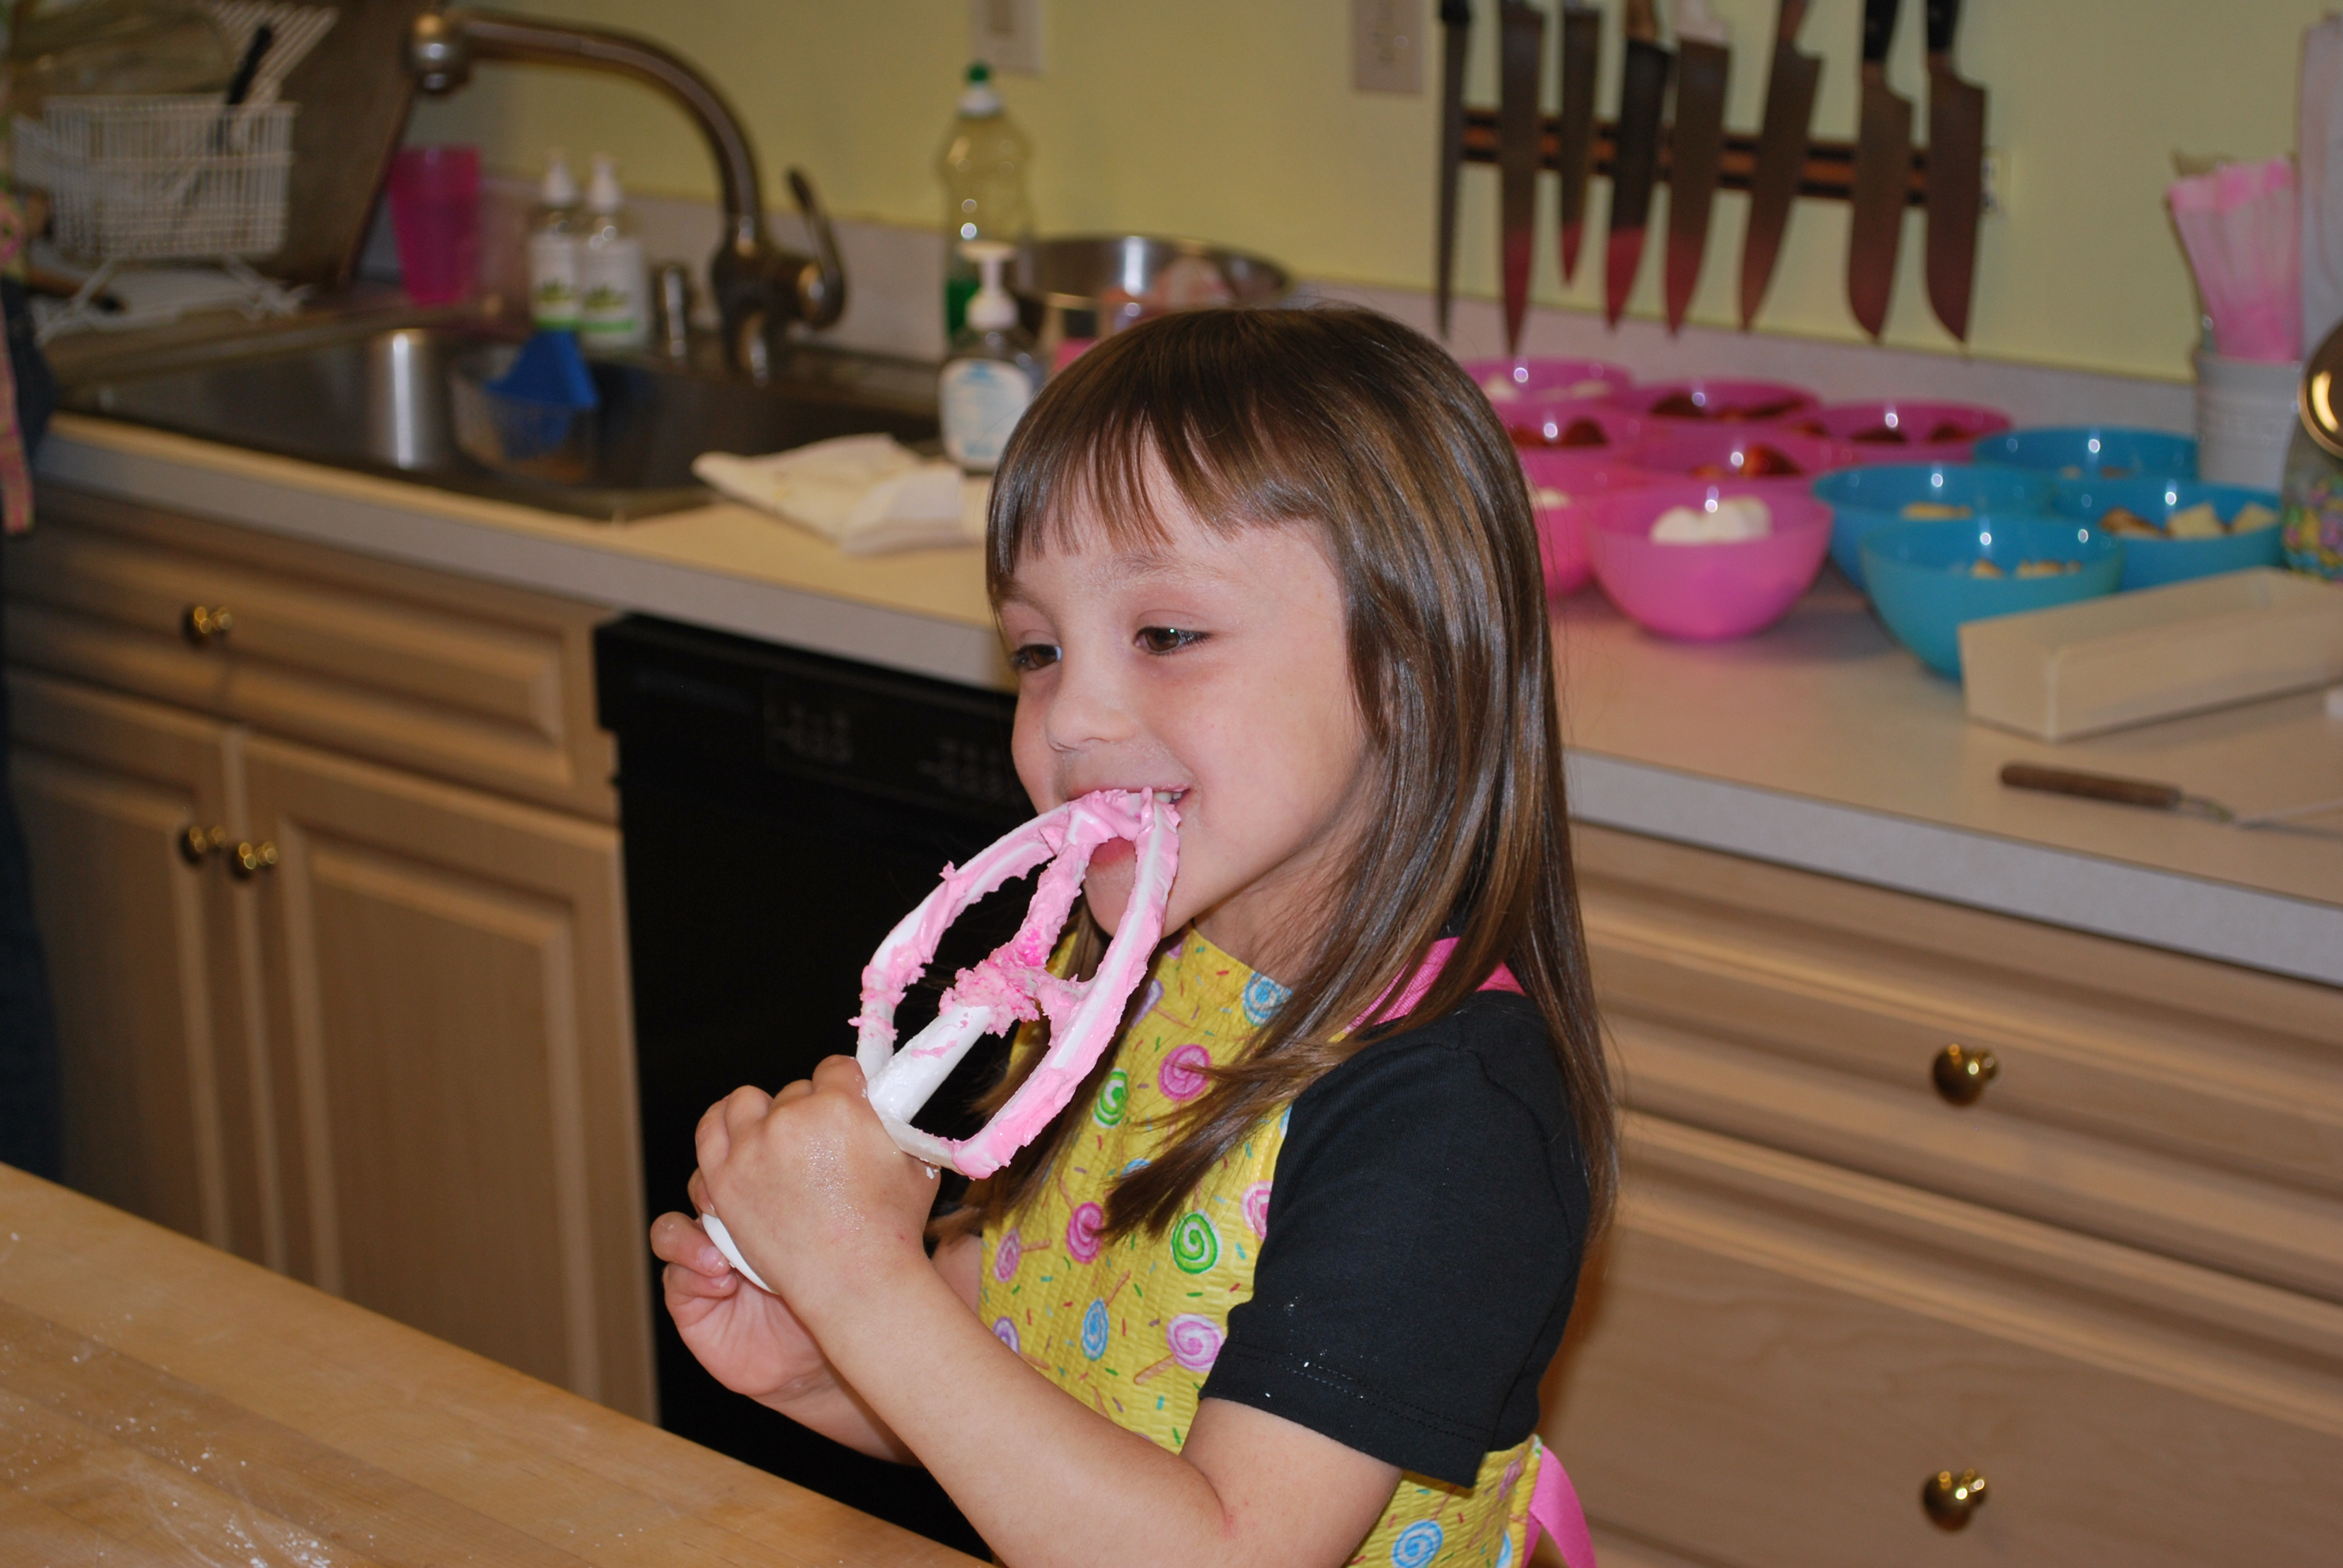
\includegraphics{DSC_0165.jpg}

``Jess's Cookbook'' is your ultimate guide to creating delicious and
memorable meals for every occasion. Packed with a variety of recipes for
breakfast, lunch, dinner, and desserts, this book offers something for
everyone, from classic favorites to creative culinary twists. Whether
you're a seasoned chef or a beginner in the kitchen, you'll find
easy-to-follow instructions, helpful tips, and precise measurements to
ensure success with every dish. The cookbook also features a
comprehensive Measurements and Conversions section, making it easier
than ever to adapt recipes to your needs. Get ready to elevate your
cooking skills and bring joy to the table with every bite!

\chapter*{Measurements and
Conversions}\label{measurements-and-conversions}
\addcontentsline{toc}{chapter}{Measurements and Conversions}

\section*{Temperature Conversions}\label{temperature-conversions}
\addcontentsline{toc}{section}{Temperature Conversions}

\begin{longtable}[]{@{}lll@{}}
\toprule\noalign{}
\textbf{Fahrenheit (°F)} & \textbf{Celsius (°C)} & \textbf{Gas Mark} \\
\midrule\noalign{}
\endhead
\bottomrule\noalign{}
\endlastfoot
500 & 260 & 10 \\
473 & 245 & 9 \\
446 & 230 & 8 \\
428 & 220 & 7 \\
392 & 200 & 6 \\
374 & 190 & 5 \\
347 & 175 & 4 \\
329 & 165 & 3 \\
302 & 150 & 2 \\
275 & 135 & 1 \\
248 & 120 & 1/2 \\
\end{longtable}

Use this online calculator to convert temperatures:

\begin{itemize}
\tightlist
\item
  \href{https://www.unitconverters.net/temperature-converter.html}{Temperature
  Conversion Calulator}
\end{itemize}

\begin{center}\rule{0.5\linewidth}{0.5pt}\end{center}

\section*{Dry Weights}\label{dry-weights}
\addcontentsline{toc}{section}{Dry Weights}

\begin{longtable}[]{@{}lllll@{}}
\toprule\noalign{}
Measurement & Cups & Ounces & Grams & Pounds \\
\midrule\noalign{}
\endhead
\bottomrule\noalign{}
\endlastfoot
1 Tablespoon & 1/16 & 1/2 oz & 15 g & / \\
2 Tablespoons & 1/8 & 1 oz & 28 g & / \\
4 Tablespoons & 1/4 & 2 oz & 57 g & / \\
8 Tablespoons & 1/2 & 4 oz & 115 g & 1/4 lb \\
16 Tablespoons & 1 & 8 oz & 227 g & 1/2 lb \\
32 Tablespoons & 2 & 16 oz & 455 g & 1 lb \\
\end{longtable}

Find these tools useful for converting dry ingredient weights:

\begin{itemize}
\tightlist
\item
  \href{https://goodcalculators.com/cooking-conversion-calculator/}{Cooking
  Measurement Conversion Calculator}
\item
  \href{https://www.inchcalculator.com/cooking-conversion-calculator/}{Cooking
  Conversion Calculator}
\end{itemize}

\begin{center}\rule{0.5\linewidth}{0.5pt}\end{center}

\section*{Liquid Volumes}\label{liquid-volumes}
\addcontentsline{toc}{section}{Liquid Volumes}

\begin{longtable}[]{@{}llllll@{}}
\toprule\noalign{}
Fluid Ounces & Tablespoons & Cups & Milliliters & Pints & Quarts \\
\midrule\noalign{}
\endhead
\bottomrule\noalign{}
\endlastfoot
1 fl oz & 2 tsp & 1/8 & 30 ml & / & / \\
2 fl oz & 4 tbsp & 1/4 & 60 ml & / & / \\
4 fl oz & 8 tbsp & 1/2 & 120 ml & / & / \\
8 fl oz & 16 tbsp & 1 & 240 ml & 1/2 pt & / \\
16 fl oz & 32 tbsp & 2 & 480 ml & 1 pt & / \\
32 fl oz & 64 tbsp & 4 & 950 ml & 2 pt & 1 qt \\
\end{longtable}

Use these tools to convert between different liquid measurements:

\begin{itemize}
\tightlist
\item
  \href{https://goodcalculators.com/cooking-conversion-calculator/}{Cooking
  Measurement Conversion Calculator}
\item
  \href{https://www.inchcalculator.com/cooking-conversion-calculator/}{Cooking
  Conversion Calculator}
\end{itemize}

\begin{center}\rule{0.5\linewidth}{0.5pt}\end{center}

\section*{Ingredient Conversions}\label{ingredient-conversions}
\addcontentsline{toc}{section}{Ingredient Conversions}

\begin{longtable}[]{@{}lll@{}}
\toprule\noalign{}
\textbf{Ingredient} & \textbf{Volume} & \textbf{Weight (grams)} \\
\midrule\noalign{}
\endhead
\bottomrule\noalign{}
\endlastfoot
All Purpose Flour & 1 Cup & 125 g \\
Granulated Sugar & 1 Cup & 200 g \\
Butter & 1 Cup & 225 g \\
Chocolate Chips & 1 Cup & 175 g \\
Cocoa Powder & 1 Cup & 85 g \\
Powdered Sugar & 1 Cup & 120 g \\
\end{longtable}

Find accurate ingredient conversions with these tools:

\begin{itemize}
\tightlist
\item
  \href{https://www.omnicalculator.com/food/cooking-measurement}{Cooking
  Measurement Converter}
\item
  \href{https://goodcalculators.com/cooking-conversion-calculator/}{Cooking
  Measurement Conversion Calculator}
\end{itemize}

\begin{center}\rule{0.5\linewidth}{0.5pt}\end{center}

\chapter{Breakfast Recipes}\label{breakfast-recipes}

\section*{Avocado Toast w/ Egg}\label{avocado-toast-w-egg}
\addcontentsline{toc}{section}{Avocado Toast w/ Egg}

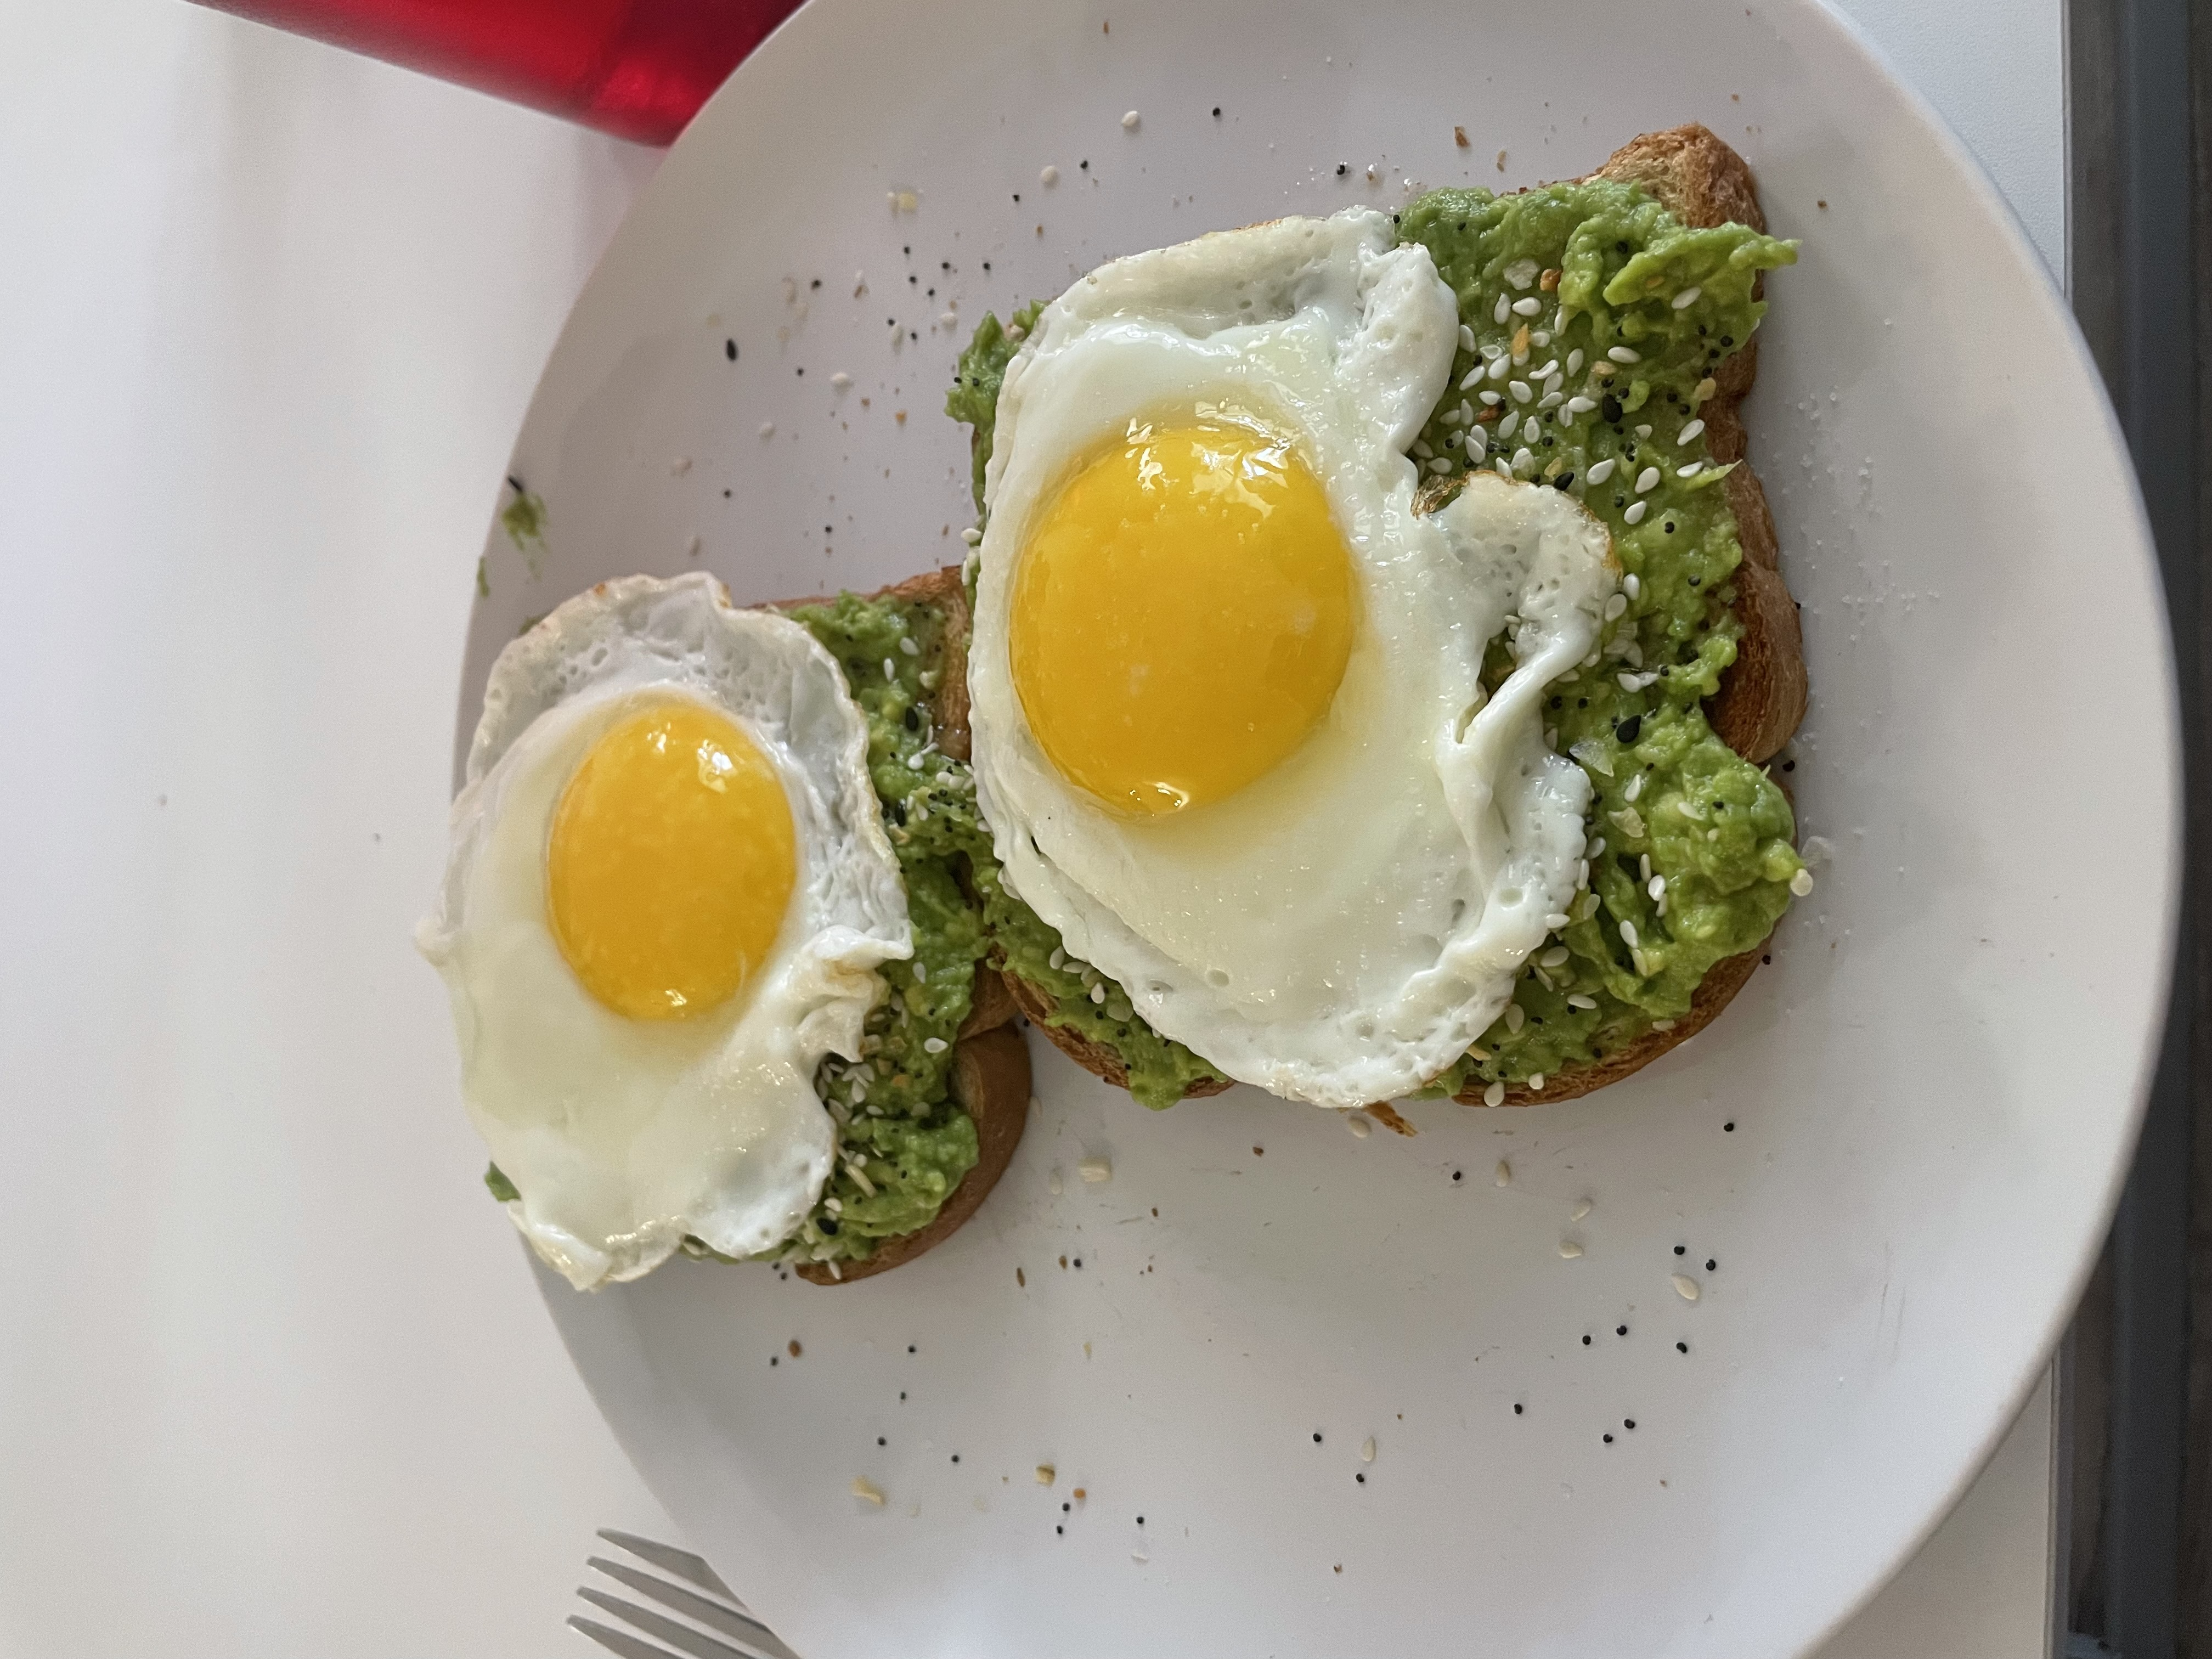
\includegraphics{atwe.jpg}

\begin{longtable}[]{@{}llll@{}}
\toprule\noalign{}
\textbf{PREP TIME} & \textbf{COOK TIME} & \textbf{SERVINGS} &
\textbf{RATING} \\
\midrule\noalign{}
\endhead
\bottomrule\noalign{}
\endlastfoot
5 mins & 5 mins & \textbf{1} & ★ ★ ★ ★ ★ \\
\end{longtable}

\subsection*{Equipment}\label{equipment}
\addcontentsline{toc}{subsection}{Equipment}

\begin{itemize}
\tightlist
\item
  1 mixing bowl
\item
  1 fork
\item
  1 sharp knife
\item
  1 skillet
\item
  Toaster
\end{itemize}

\subsection*{Ingredients}\label{ingredients}
\addcontentsline{toc}{subsection}{Ingredients}

\begin{itemize}
\tightlist
\item
  1 ripe avocado
  \href{https://www.publix.com/pd/hass-avocados/RIO-PCI-107578?origin=search1}{*}
\item
  1 lemon wedge
  \href{https://www.publix.com/pd/lemons/RIO-PCI-107591?origin=search1}{*}
\item
  Salt
  \href{https://www.publix.com/pd/morton-salt/RIO-PCI-103677?origin=search9}{*}
\item
  Pepper
  \href{https://www.publix.com/pd/publix-black-pepper-ground/RIO-PCI-110488?origin=search1}{*}
\item
  Everything bagel seasoning
  \href{https://www.publix.com/pd/badia-everything-bagel/RIO-PCI-572577?origin=search1}{*}
\item
  2 pieces of toast
  \href{https://www.publix.com/pd/natures-own-honey-wheat-sandwich-bread-20-oz-loaf/RIO-PCI-144911?origin=search1}{*}
\item
  2 eggs
  \href{https://www.publix.com/pd/publix-eggs-large/RIO-PCI-145492?origin=search8}{*}
\item
  2 tbsp avocado oil
  \href{https://www.publix.com/pd/publix-avocado-oil/RIO-PCI-575036?origin=search1}{*}
\end{itemize}

Click on the '*' next to each ingredient to see detailed information and
resources for it.

Instructions

\textbf{Step 1:} Halve the avocado vertically and remove the pit. Use a
small knife to dice the avocado flesh while it's still inside the skin.
Scoop the diced avocado flesh out of the skin and into a small bowl.

\textbf{Step 2:} Use a fork to mash the avocado until it's as smooth as
you like it. Mix in a pinch of salt and pepper (about 1/8 teaspoon each)
and add more to taste, if desired. Lastly, squeeze in the lemon juice
and mix thoroughly.

\textbf{Step 3:} Toast your slice of bread until golden and firm.

\textbf{Step 4:} While the bread toasts cook the egg by first pouring 1
tbsp of avocado oil over low heat in a small (8-inch) non-stick skillet.
Once it is hot, crack the eggs into the skillet and cook the egg until
it is cooked through, about 2 to 3 minutes.

\textbf{Step 5:} Once the toast is done, spread the avocado mash on top
of each slice. Drizzle them both with avocado oil and sprinkle them with
everything bagel seasoning.

\textbf{Step 6:} Once the eggs are done, place the eggs on each of the
slices and enjoy!

\section*{French Toast}\label{french-toast}
\addcontentsline{toc}{section}{French Toast}

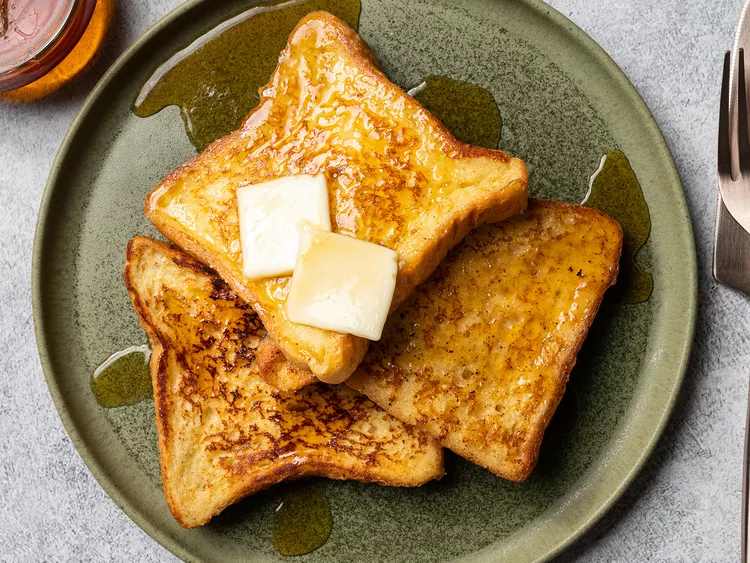
\includegraphics{ft.jpg}

\begin{longtable}[]{@{}llll@{}}
\toprule\noalign{}
\textbf{PREP TIME} & \textbf{COOK TIME} & \textbf{SERVINGS} &
\textbf{RATING} \\
\midrule\noalign{}
\endhead
\bottomrule\noalign{}
\endlastfoot
5 mins & 35 mins & \textbf{4} & ★ ★ ★ ★ ☆ \\
\end{longtable}

\subsection*{Equipment}\label{equipment-1}
\addcontentsline{toc}{subsection}{Equipment}

\begin{itemize}
\tightlist
\item
  1 rimmed baking sheet
\item
  1 wire rack
\item
  1 large mixing bowl
\item
  1 large non-stick skillet
\end{itemize}

\subsection*{Ingredients}\label{ingredients-1}
\addcontentsline{toc}{subsection}{Ingredients}

\begin{itemize}
\tightlist
\item
  8 (1/2-inch thick) slices of white bread
  \href{https://www.publix.com/pd/natures-own-honey-wheat-sandwich-bread-20-oz-loaf/RIO-PCI-144911?origin=search1}{*}
\item
  6 large eggs
  \href{https://www.publix.com/pd/publix-eggs-large/RIO-PCI-145492?origin=search8}{*}
\item
  4 tbsp sugar, plus more for sprinkling
  \href{https://www.publix.com/pd/publix-sugar-pure-granulated-extra-fine/RIO-PCI-143101?origin=search1}{*}
\item
  Pinch of salt
  \href{https://www.publix.com/pd/morton-salt/RIO-PCI-103677?origin=search9}{*}
\item
  Pinch of ground cinnamon
  \href{https://www.publix.com/pd/publix-cinnamon-ground/RIO-PCI-111220?origin=search1}{*}
\item
  Pinch of freshly grated nutmeg
  \href{https://www.publix.com/pd/mccormick-ground-nutmeg/RIO-PCI-110645?origin=search1}{*}
\item
  1/4 teaspoon vanilla extract
  \href{https://www.publix.com/pd/publix-vanilla-extract/RIO-PCI-110432?origin=search1}{*}
\item
  2 cups whole milk
  \href{https://www.publix.com/pd/publix-milk-whole/RIO-PCI-120772?origin=search3}{*}
\item
  4 tbsp unsalted butter for the pan
  \href{https://www.publix.com/pd/land-o-lakes-unsalted-butter-made-with-sweet-cream/RIO-PCI-112513?origin=search2}{*}
\item
  Maple syrup, for serving
  \href{https://www.publix.com/pd/pearl-milling-company-syrup-original/RIO-PCI-102438?origin=search10}{*}
\end{itemize}

Click on the '*' next to each ingredient to see detailed information and
resources for it.

Instructions

\textbf{Step 1:} Set a wire rack on a rimmed baking sheet in the oven
and preheat to 200°F (93°C). If using very fresh, moist bread, arrange
slices in a single layer on the rack and cook in oven, turning once,
until lightly toasted, about 10 minutes.

\textbf{Step 2:} Meanwhile, in a large mixing bowl, whisk together eggs,
sugar, salt, cinnamon, nutmeg, and vanilla until thoroughly combined.
Add milk and whisk to blend.

\textbf{Step 3:} Heat 1 tablespoon butter in a large non-stick or cast
iron skillet over medium heat, swirling skillet, until foaming subsides,
about 5 minutes.

\textbf{Step 4:} Soak 2 slices of bread in egg bath, turning, until
saturated. Add soaked bread to skillet and cook, swirling occasionally,
until browned on bottom side, about 3 minutes. Sprinkle top side of
bread with sugar, flip, and continue to cook, swirling occasionally,
until browned on second side, about 3 minutes longer.

\textbf{Step 5:} Transfer French toast to the rack in the oven in a
single layer to keep warm and repeat with remaining slices of bread and
egg bath.

\textbf{Step 6:} Serve French toast with pats of butter and maple syrup.

\chapter{Lunch Recipes}\label{lunch-recipes}

\section*{Salmon Rice Bowl}\label{salmon-rice-bowl}
\addcontentsline{toc}{section}{Salmon Rice Bowl}

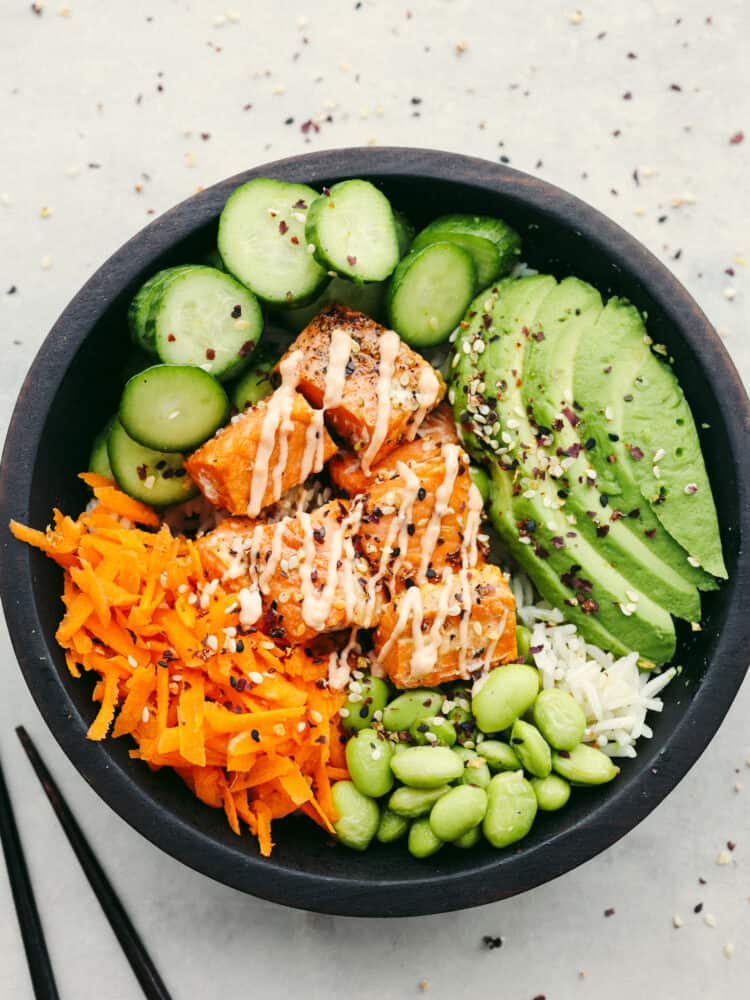
\includegraphics{sb.jpg}

\begin{longtable}[]{@{}llll@{}}
\toprule\noalign{}
\textbf{PREP TIME} & \textbf{COOK TIME} & \textbf{SERVINGS} &
\textbf{RATING} \\
\midrule\noalign{}
\endhead
\bottomrule\noalign{}
\endlastfoot
10 mins & 30 mins & \textbf{1} & ★ ★ ★ ★ ★ \\
\end{longtable}

\subsection*{Equipment}\label{equipment-2}
\addcontentsline{toc}{subsection}{Equipment}

\begin{itemize}
\tightlist
\item
  1 large cooking pot
\item
  1 airfryer or large skillet
\item
  1 sharp knife
\item
  1 rubber spatula
\item
  1 cutting board
\item
  2 small mixing bowls
\end{itemize}

\subsection*{Ingredients}\label{ingredients-2}
\addcontentsline{toc}{subsection}{Ingredients}

\begin{itemize}
\tightlist
\item
  1 cup of jasmine rice
  \href{https://www.publix.com/pd/publix-rice-jasmine/RIO-PCI-142398?origin=search1}{*}
\item
  1 1/4 cups water (cold tap water)
\item
  4 ounces salmon filet
  \href{https://www.publix.com/pd/salmon-select-cuts-fresh-responsibly-sourced-farmed/RIO-FNU-591951?origin=search2}{*}
\item
  1/2 tsp of salt
  \href{https://www.publix.com/pd/morton-salt/RIO-PCI-103677?origin=search9}{*}
\item
  1/4 tsp of pepper
  \href{https://www.publix.com/pd/publix-black-pepper-ground/RIO-PCI-110488?origin=search1}{*}
\item
  1/4 tsp onion powder
  \href{https://www.publix.com/pd/publix-onion-powder/RIO-PCI-111136?origin=search1}{*}
\item
  1/2 avocado (sliced or diced)
  \href{https://www.publix.com/pd/hass-avocados/RIO-PCI-107578?origin=search1}{*}
\item
  1/4 carrots (shredded)
  \href{https://www.publix.com/pd/greenwise-shredded-carrots-organic/RIO-PCI-107793?origin=search1}{*}
\item
  1/4 cup Edamame (cooked)
  \href{https://www.publix.com/pd/seapoint-farms-edamame/RIO-PCI-159631?origin=search1}{*}
\item
  1 tbsp soy sauce
  \href{https://www.publix.com/pd/publix-sauce-soy-less-sodium/RIO-PCI-125220?origin=search1}{*}
\item
  4 tsp Sriracha mayo
  \href{https://www.publix.com/pd/lee-kum-kee-dressingspread-mayo-sriracha/RIO-PCI-520244?origin=search4}{*}
\item
  Sesame Seeds
  \href{https://www.publix.com/pd/badia-sesame-seeds-tri-color-organic/RIO-PCI-543666?origin=search3}{*}
\end{itemize}

Click on the '*' next to each ingredient to see detailed information and
resources for it.

Instructions

\textbf{Step 1:} Place rice and water in a medium saucepan (one with a
tight fitting lid). Bring to rapid simmer with NO LID on medium high.

\textbf{Step 2:} Turn down to low or medium low so it's simmering
gently, then place lid on. Do not lift lid during cook.

\textbf{Step 3:} Cook 12 minutes or until water is absorbed by rice -
tilt pot to check (if lid not glass, then QUICKLY lift lid to check)

\textbf{Step 4:} Keep the lid on then remove from heat. Stand 10
minutes, then fluff with rubber spatula or rice paddle.

\textbf{Step 5:} Preheat the air fryer to 390 degrees Farhenheit. Remove
the skin from the salmon filets and cut the salmon into 1 inch cubes.

\textbf{Step 6:} Place the cubed salmon in a bowl and season with salt,
pepper, and onion powder.

\textbf{Step 7:} Place the salmon in the air fryer basket in a single
layer and cook for 6-8 minutes, or until the internal temperature has
reached 125 degrees Fahrenheit. Feel free to pan fry over medium-high
heat in a skillet for the same amount of time if you prefer.

\textbf{Step 8:} Place the cooked rice in the bowl first. Layer on the
cooked salmon, avocado, cucumber, and edamame.

\textbf{Step 9:} Drizzle on the soy sauce, Sriracha mayo, and garnish
with sesame seeds.

\section*{Turkey Sandwich}\label{turkey-sandwich}
\addcontentsline{toc}{section}{Turkey Sandwich}

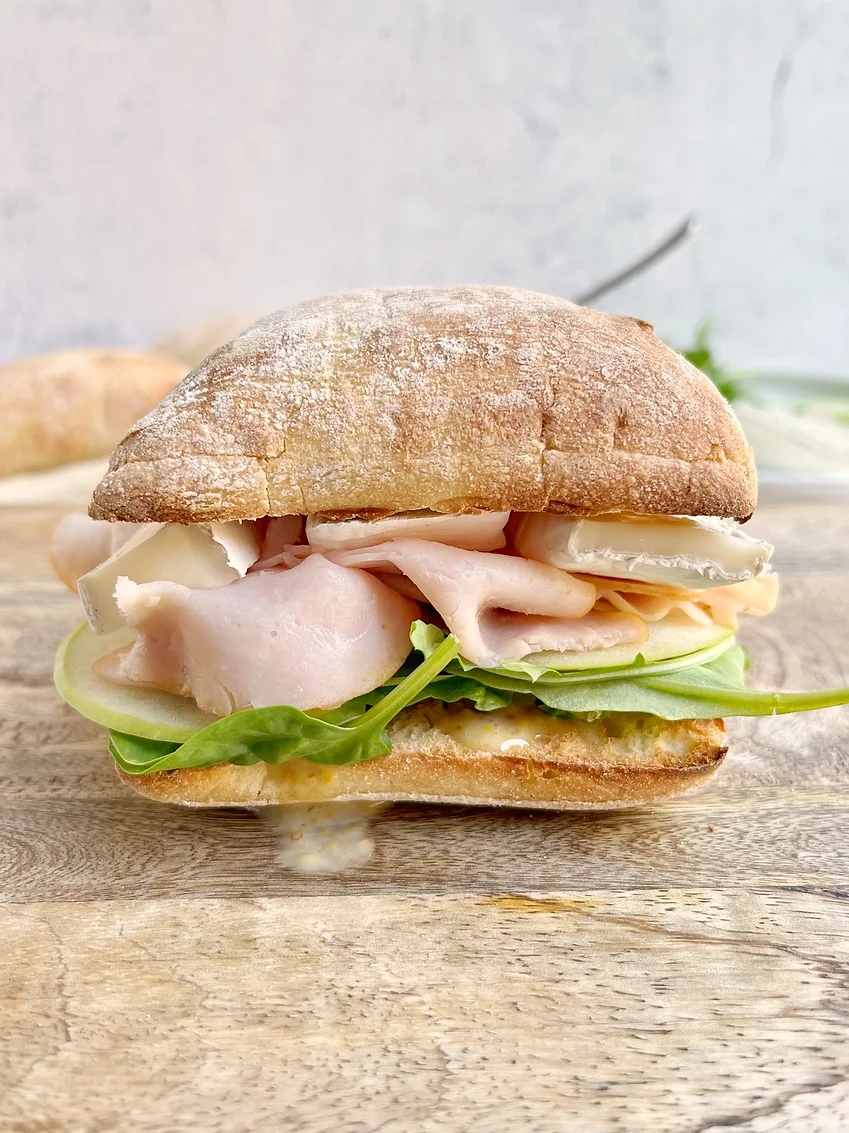
\includegraphics{ts.jpg}

\begin{longtable}[]{@{}llll@{}}
\toprule\noalign{}
\textbf{PREP TIME} & \textbf{COOK TIME} & \textbf{SERVINGS} &
\textbf{RATING} \\
\midrule\noalign{}
\endhead
\bottomrule\noalign{}
\endlastfoot
5 mins & 7 mins & \textbf{1} & ★ ★ ★ ★ ★ \\
\end{longtable}

\subsection*{Equipment}\label{equipment-3}
\addcontentsline{toc}{subsection}{Equipment}

\begin{itemize}
\tightlist
\item
  1 airfryer
\item
  1 sharp knife
\end{itemize}

\subsection*{Ingredients}\label{ingredients-3}
\addcontentsline{toc}{subsection}{Ingredients}

\begin{itemize}
\tightlist
\item
  1 ciabatta bread
  \href{https://www.publix.com/pd/presliced-ciabatta-rolls-4-count/RIO-PCI-282539?origin=search1}{*}
\item
  2 tbsp of mayonnaise
  \href{https://www.publix.com/pd/hellmanns-real-mayonnaise-real-mayo-squeeze-bottle/RIO-PCI-509942?origin=search2}{*}
\item
  1 half of an avocado
  \href{https://www.publix.com/pd/hass-avocados/RIO-PCI-107578?origin=search1}{*}
\item
  1/2 cup of shredded lettuce
  \href{https://www.publix.com/pd/fresh-express-garden-salad-shreds-iceberg/RIO-PCI-107853?origin=search1}{*}
\item
  2 slices of provolone cheese
  \href{https://www.publix.com/pd/publix-not-smoked-provolone-cheese-slices/RIO-PCI-136662?origin=search3}{*}
\item
  2 tbsp olive oil
  \href{https://www.publix.com/pd/publix-olive-oil-extra-virgin/RIO-PCI-103897?origin=search1}{*}
\item
  3 slices of Boar's Head Ovengold Roasted Turkey
  \href{https://www.publix.com/pd/boars-head-ovengold-roasted-turkey-breast/RIO-DSM-100234?origin=search1}{*}
\end{itemize}

Click on the '*' next to each ingredient to see detailed information and
resources for it.

Instructions

\textbf{Step 1:} Slice the ciabatta bread in half. Drizzle the olive oil
evenly on both slices.

\textbf{Step 2:} Preheat the air fryer to 350 degrees Farhenheit. Once
heated, place both slices in the air fryer basket in a single layer and
cook for 5 minutes.

\textbf{Step 3:} Remove the slices from the air fryer once the 5 minutes
are up. Spread the mayonnaise evenly on both slices.

\textbf{Step 4:} Assemble the sandwich: Layer each half of the bread
with one slice of provolone cheese. On the bottom half, place the three
slices of turkey evenly. Then top the turkey with the shredded lettuce
and the sliced avocado. Close the sandwiches with the top roll, and
enjoy.

\chapter{Dinner Recipes}\label{dinner-recipes}

\section*{Garlic Parmesan Steak
Pasta}\label{garlic-parmesan-steak-pasta}
\addcontentsline{toc}{section}{Garlic Parmesan Steak Pasta}

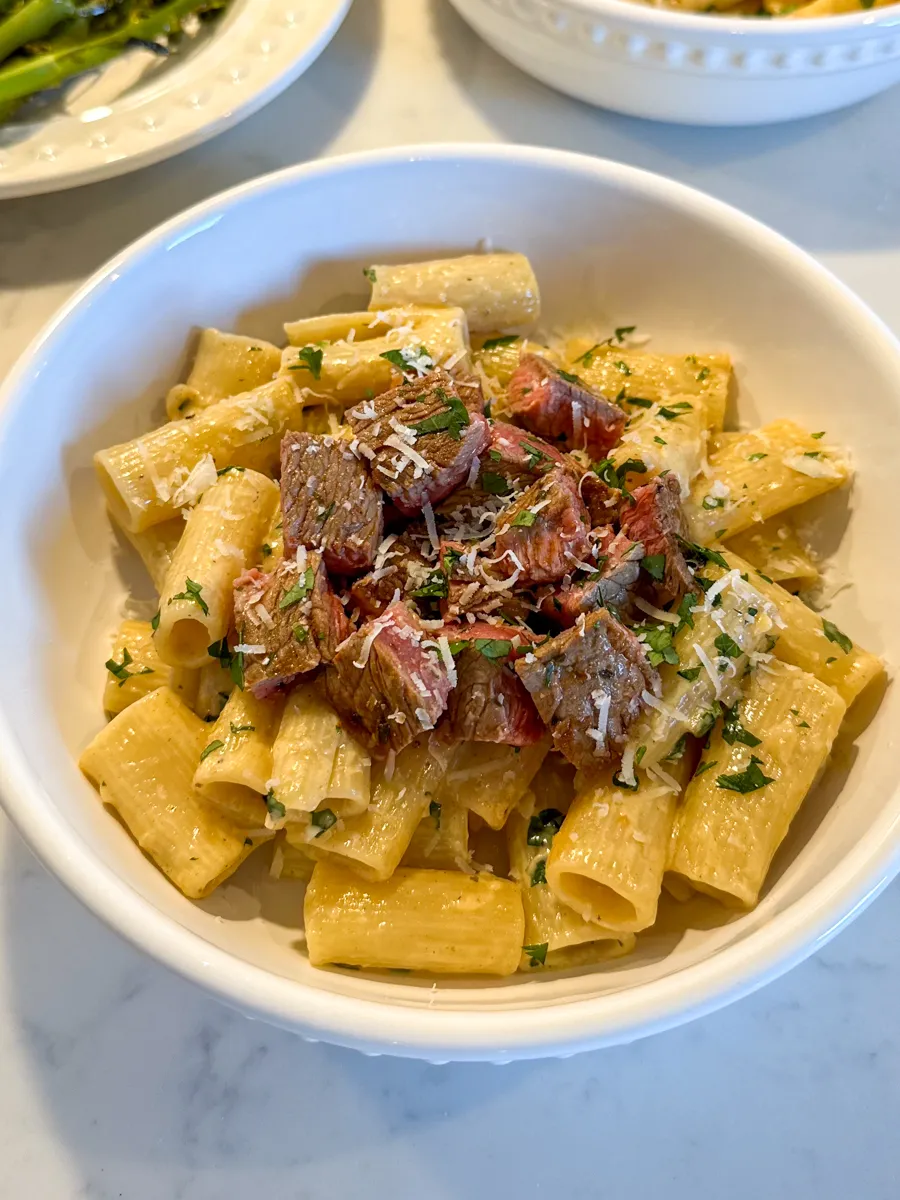
\includegraphics{gpsp.jpg}

\begin{longtable}[]{@{}llll@{}}
\toprule\noalign{}
\textbf{PREP TIME} & \textbf{COOK TIME} & \textbf{SERVINGS} &
\textbf{RATING} \\
\midrule\noalign{}
\endhead
\bottomrule\noalign{}
\endlastfoot
5 mins & 20 mins & \textbf{4} & ★ ★ ★ ★ ★ \\
\end{longtable}

\subsection*{Equipment}\label{equipment-4}
\addcontentsline{toc}{subsection}{Equipment}

\begin{itemize}
\tightlist
\item
  2 cutting boards
\item
  1 frying pan
\item
  1 sharp knife
\item
  1 large pot
\end{itemize}

\subsection*{Ingredients}\label{ingredients-4}
\addcontentsline{toc}{subsection}{Ingredients}

\begin{itemize}
\tightlist
\item
  450 g Ribeye Steak (approx. 2 steaks)
  \href{https://www.publix.com/pd/ribeye-steaks-boneless-thin-sliced-publix-usda-choice-beef/RIO-PCI-119976?origin=search3}{*}
\item
  1 tbsp paprika
  \href{https://www.publix.com/pd/publix-paprika-ground/RIO-PCI-123196?origin=search1}{*}
\item
  2 tbsp olive oil
  \href{https://www.publix.com/pd/publix-olive-oil-extra-virgin/RIO-PCI-103897?origin=search1}{*}
\item
  2 tsp dried parsley
  \href{https://www.publix.com/pd/publix-parsley-flakes/RIO-PCI-111166?origin=search1}{*}
\item
  Salt
  \href{https://www.publix.com/pd/morton-salt/RIO-PCI-103677?origin=search9}{*}
\item
  Pepper
  \href{https://www.publix.com/pd/publix-black-pepper-ground/RIO-PCI-110488?origin=search1}{*}
\item
  1 onion
  \href{https://www.publix.com/pd/white-onions-jumbo/RIO-PCI-107142?origin=search3}{*}
\item
  3 cloves of garlic
  \href{https://www.publix.com/pd/garlic/RIO-PCI-107127?origin=search1}{*}
\item
  2 tbsp butter
  \href{https://www.publix.com/pd/land-o-lakes-salted-butter-sticks/RIO-PCI-112640?origin=search2}{*}
\item
  1/2 cup chicken stock
  \href{https://www.publix.com/pd/swanson-unsalted-chicken-stock/RIO-PCI-134444?origin=search1}{*}
\item
  1/2 cup double cream
  \href{https://www.publix.com/pd/devon-cream-double-cream-english/RIO-PCI-114706?origin=search1}{*}
\item
  1/2 cup Parmesan cheese
  \href{https://www.publix.com/pd/publix-parmesan-fancy-shredded-cheese/RIO-PCI-132616?origin=search6}{*}
\item
  1/3 cup fresh parsley
  \href{https://www.publix.com/pd/thats-tasty-italian-parsley/RIO-PCI-574065?origin=search4}{*}
\item
  300 g Rigatoni pasta
  \href{https://www.publix.com/pd/ronzoni-rigatoni-pasta-16-oz-large-ribbed-tubes-non-gmo/RIO-PCI-100730?origin=search4}{*}
\end{itemize}

Click on the '*' next to each ingredient to see detailed information and
resources for it.

Instructions

\textbf{Step 1:} Start by generously seasoning both sides of the ribeye
steaks with paprika, dried parsley, salt, and pepper. Drizzle with olive
oil and rub the seasonings into the meat to ensure even coverage. Set
aside to allow the flavors to penetrate the steak.

\textbf{Step 2:} While the steaks rest, finely dice the onion, mince the
garlic cloves, finely chop the fresh parsley, and grate the Parmesan
cheese.

\textbf{Step 3:} Heat a frying pan over high heat for about 1 minute to
ensure it's hot enough to sear the steaks properly.

\textbf{Step 4:} Place the steak on the frying pan and fry on high heat
for 1 minute until browned, flip over and fry for 1 minute on the other
side then add 1 tablespoon butter, spoon the butter over the steak for a
further minute then set aside to rest.

\textbf{Step 5:} Add 1 tablespoon of butter to the pan and spoon the
melted butter over the steaks for an additional minute.

\textbf{Step 6:} Remove the steaks from the pan and set them aside to
rest (cooking times may vary depending on pan and type of cooker as well
as how pink you like your steak).

\textbf{Step 7:} Once the steaks have been set aside, bring the pasta to
the boil by adding table salt to a pot of boiling water. Once the pot of
water is boiling, add in the pasta and continue to boil.

\textbf{Step 8:} While the pasta is cooking, begin making the sauce in
the same pan the steaks were cooked in. Add more butter along with an
onion and fry for 5 minutes, i also like to add a little more paprika at
this point but this is optional. Add the garlic and fry for a further
minute.

\textbf{Step 9:} While the pasta is cooking, begin making the sauce in
the same pan the steaks were cooked in. Add more butter along with an
onion and fry for 5 minutes, i also like to add a little more paprika at
this point but this is optional. Add the garlic and fry for a further
minute.

\textbf{Step 10:} Add the chicken stock and double cream to the mixture
and cook on medium-high heat for 2-3 minutes before adding the Parmesan
and stirring together, reduce to a simmer. Add pasta water as desired to
loosen the sauce.

\textbf{Step 11:} Add in the pasta and chopped parsley, stirring to
combine before cutting the steaks in to cubes to be placed on top of
each serving of pasta.

\section*{Brie\&Bacon Smash Burger
Tacos}\label{briebacon-smash-burger-tacos}
\addcontentsline{toc}{section}{Brie\&Bacon Smash Burger Tacos}

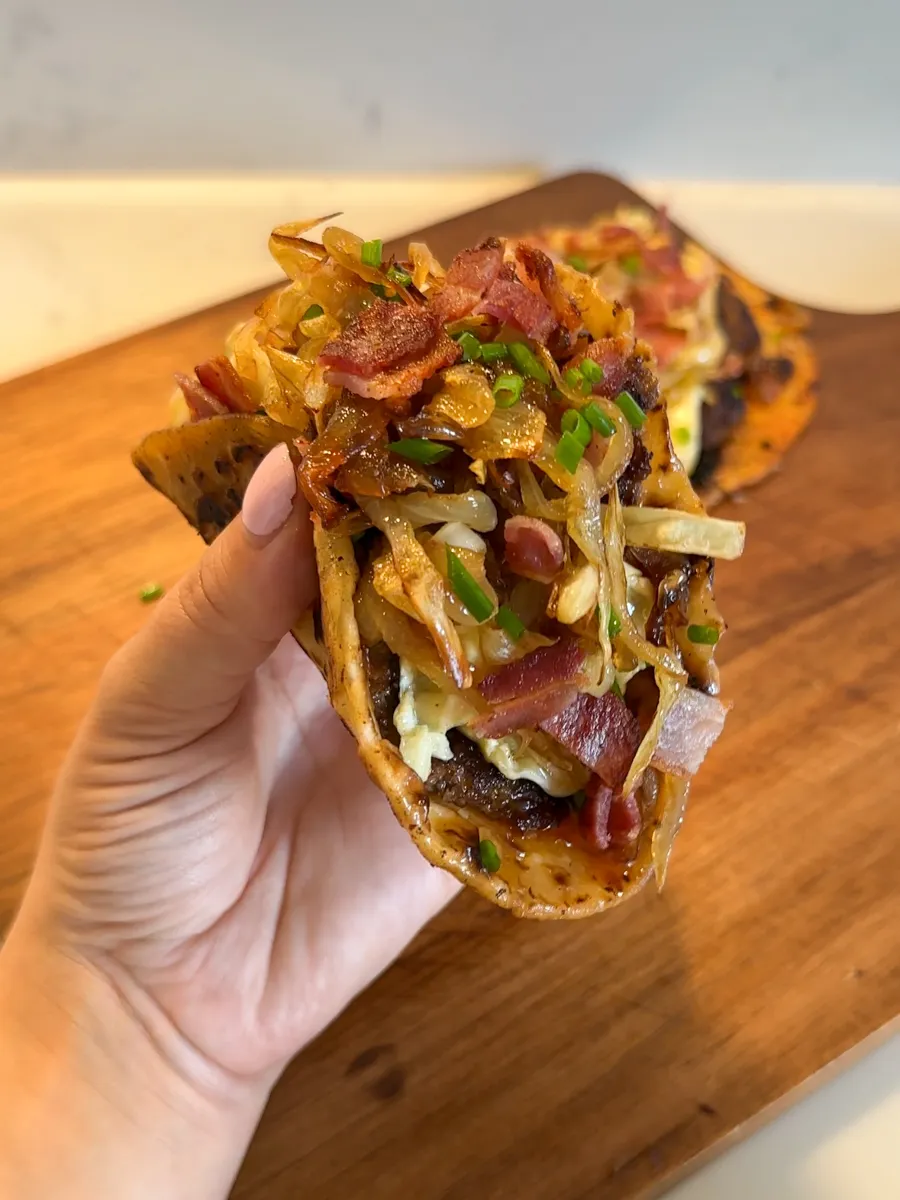
\includegraphics{bbsb.jpg}

\begin{longtable}[]{@{}llll@{}}
\toprule\noalign{}
\textbf{PREP TIME} & \textbf{COOK TIME} & \textbf{SERVINGS} &
\textbf{RATING} \\
\midrule\noalign{}
\endhead
\bottomrule\noalign{}
\endlastfoot
10 mins & 35 mins & \textbf{4} & ★ ★ ★ ★ ☆ \\
\end{longtable}

\subsection*{Equipment}\label{equipment-5}
\addcontentsline{toc}{subsection}{Equipment}

\begin{itemize}
\tightlist
\item
  1 large skillet
\item
  1 large mixing bowl
\item
  1 spatula
\item
  Paper towels
\end{itemize}

\subsection*{Ingredients}\label{ingredients-5}
\addcontentsline{toc}{subsection}{Ingredients}

\begin{itemize}
\tightlist
\item
  500 g beef mince
  \href{https://www.publix.com/pd/lean-ground-beef-burgers-7-fat-publix-beef-usda-inspected/RIO-PCI-117504?origin=search13}{*}
\item
  8 mini tortillas
  \href{https://www.publix.com/pd/mission-flour-tortillas-street-tacos/RIO-PCI-563292?origin=search12}{*}
\item
  1 tbsp paprika
  \href{https://www.publix.com/pd/publix-paprika-ground/RIO-PCI-123196?origin=search1}{*}
\item
  1 tsp onion powder
  \href{https://www.publix.com/pd/publix-onion-powder/RIO-PCI-111136?origin=search1}{*}
\item
  1 tsp thyme
  \href{https://www.publix.com/pd/thats-tasty-thyme/RIO-PCI-574066?origin=search2}{*}
\item
  1 tbsp olive oil
  \href{https://www.publix.com/pd/publix-olive-oil-extra-virgin/RIO-PCI-103897?origin=search1}{*}
\item
  Salt
  \href{https://www.publix.com/pd/morton-salt/RIO-PCI-103677?origin=search9}{*}
\item
  Pepper
  \href{https://www.publix.com/pd/publix-black-pepper-ground/RIO-PCI-110488?origin=search1}{*}
\item
  4 bacon rashers
  \href{https://www.publix.com/pd/hormel-black-label-bacon-original/RIO-PCI-117322?origin=search3}{*}
\item
  2 onions
  \href{https://www.publix.com/pd/white-onions-jumbo/RIO-PCI-107142?origin=search3}{*}
\item
  250 g Brie sliced
  \href{https://www.publix.com/pd/publix-deli-brie-cheese-imported-round/RIO-PCI-174121?origin=search5}{*}
\item
  1 tbsp butter
  \href{https://www.publix.com/pd/land-o-lakes-salted-butter-sticks/RIO-PCI-112640?origin=search2}{*}
\item
  2 tsp sugar
  \href{https://www.publix.com/pd/publix-sugar-pure-granulated-extra-fine/RIO-PCI-143101?origin=search1}{*}
\item
  1 tbsp chopped chives
  \href{https://www.publix.com/pd/thats-tasty-chives/RIO-PCI-574073?origin=search2}{*}
\end{itemize}

Click on the '*' next to each ingredient to see detailed information and
resources for it.

Instructions

\textbf{Step 1:} Start by preparing the onions. Thinly slice them by
cutting off the tops and bottoms, then halving them and slicing thinly
from right to left.

\textbf{Step 2:} In a pan, melt some butter and add the onions along
with a bit of sugar. Let them cook on low heat for 25-30 minutes,
stirring occasionally.

\textbf{Step 3:} While the onions are caramelizing, cook the bacon. Heat
a large frying pan with a little oil and cook the bacon rashers until
they're crispy, about 3-4 minutes per side. Once done, set them aside to
cool.

\textbf{Step 4:} In a mixing bowl, combine the beef mince with paprika,
onion granules, and dried thyme. Divide the seasoned beef into 8 equal
balls.

\textbf{Step 5:} Take each ball of beef and place it on a mini tortilla.
Using your fingers, press the beef down until it evenly covers the
tortilla.

\textbf{Step 6:} Heat a lightly greased skillet over medium heat. Place
1-2 tortillas, beef side down, onto the pan and cook for about 4
minutes, allowing the beef to brown and crisp up.

\textbf{Step 7:} Turn the heat down to medium and flip the tortillas
over with a spatula, taking care to lift and wipe any excess grease from
the pan with a paper towel to keep the tortilla from becoming soggy.

\textbf{Step 8:} Once flipped, add slices of Brie cheese on top of each
smash burger. Pour a little water into the pan and cover it with a lid
to steam the Brie for about 2 minutes.

\textbf{Step 9:} Remove the smash burger tacos from the skillet and
place them on a paper towel or a board to soak up any remaining grease.
Top each one with a generous helping of caramelized onions, crispy bacon
pieces, and a sprinkle of chopped chives.

\chapter{Dessert Recipes}\label{dessert-recipes}

\section*{Loaded Brookie}\label{loaded-brookie}
\addcontentsline{toc}{section}{Loaded Brookie}

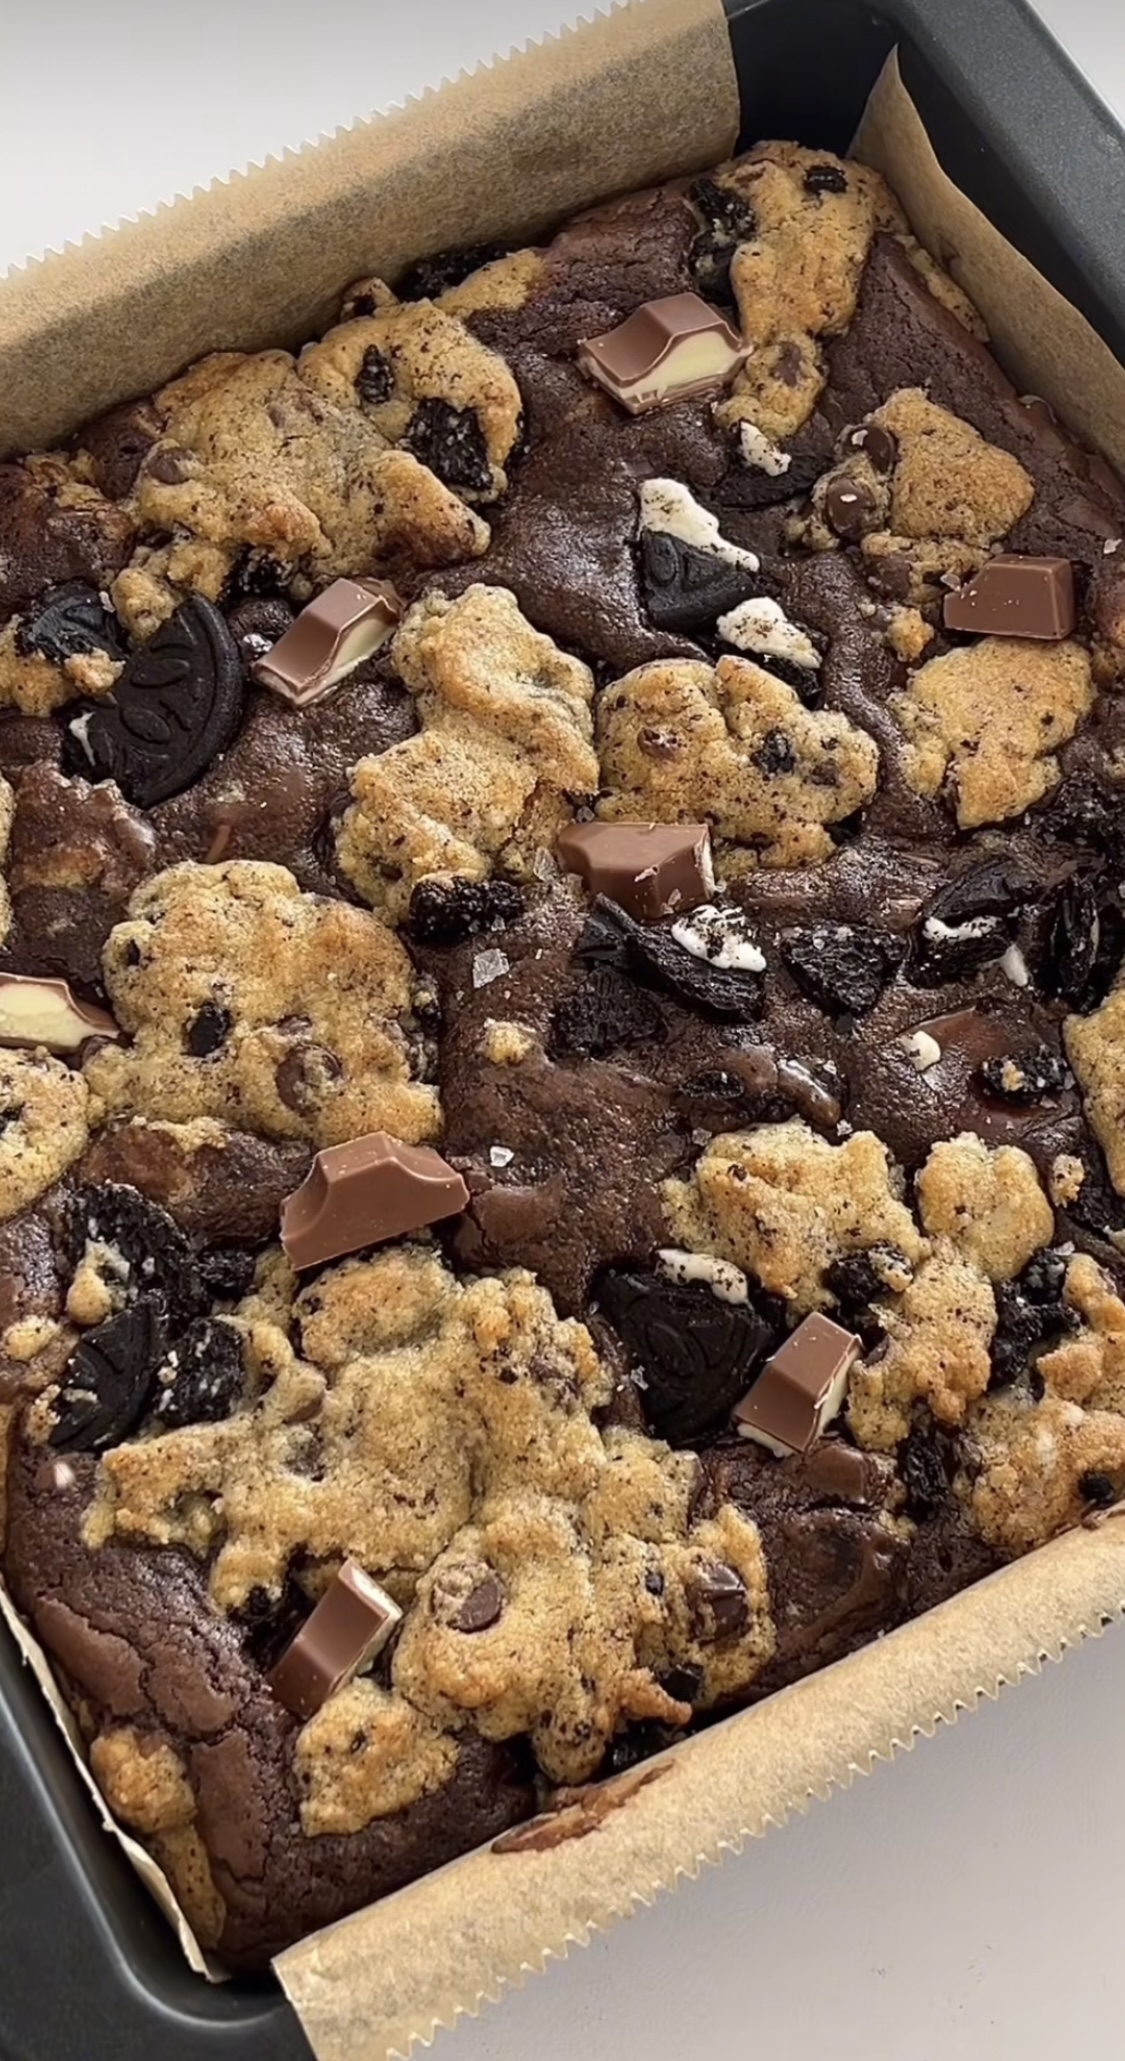
\includegraphics{lb.jpg}

\begin{longtable}[]{@{}llll@{}}
\toprule\noalign{}
\textbf{PREP TIME} & \textbf{COOK TIME} & \textbf{SERVINGS} &
\textbf{RATING} \\
\midrule\noalign{}
\endhead
\bottomrule\noalign{}
\endlastfoot
15 mins & 45 mins & \textbf{12} & ★ ★ ★ ★ ★ \\
\end{longtable}

\subsection*{Equipment}\label{equipment-6}
\addcontentsline{toc}{subsection}{Equipment}

\begin{itemize}
\tightlist
\item
  2 mixing bowls
\item
  2 whisks
\item
  1 sifter
\item
  1 square baking tin
\item
  Aluminum foil
\item
  Parchment paper
\end{itemize}

\subsection*{Ingredients}\label{ingredients-6}
\addcontentsline{toc}{subsection}{Ingredients}

Brownie Batter:

\begin{itemize}
\tightlist
\item
  100 g dark chocolate
  \href{https://www.publix.com/pd/lilys-baking-chips-dark-chocolate/RIO-PCI-541806?origin=search8}{*}
\item
  100 g unsalted butter
  \href{https://www.publix.com/pd/land-o-lakes-unsalted-butter-made-with-sweet-cream/RIO-PCI-112513?origin=search2}{*}
\item
  2 medium eggs
  \href{https://www.publix.com/pd/publix-eggs-large/RIO-PCI-145492?origin=search8}{*}
\item
  140 g caster sugar
  \href{https://www.publix.com/pd/publix-sugar-pure-granulated-extra-fine/RIO-PCI-143101?origin=search1}{*}
\item
  50 g plain flour
  \href{https://www.publix.com/pd/publix-all-purpose-flour/RIO-PCI-104014?origin=search1}{*}
\item
  25 g cocoa powder
  \href{https://www.publix.com/pd/hersheys-dutched-cocoa-special-dark/RIO-PCI-102330?origin=search1}{*}
\item
  100 g Kinder chocolate
  \href{https://www.publix.com/pd/kinder-chocolate/RIO-PCI-613809?origin=search1}{*}
\end{itemize}

Cookie Dough:

\begin{itemize}
\tightlist
\item
  115 g unsalted butter
  \href{https://www.publix.com/pd/land-o-lakes-unsalted-butter-made-with-sweet-cream/RIO-PCI-112513?origin=search2}{*}
\item
  125 g light brown sugar
  \href{https://www.publix.com/pd/publix-sugar-light-brown/RIO-PCI-128825?origin=search1}{*}
\item
  1 medium egg
  \href{https://www.publix.com/pd/publix-eggs-large/RIO-PCI-145492?origin=search8}{*}
\item
  1/2 tsp vanilla extract
  \href{https://www.publix.com/pd/publix-vanilla-extract/RIO-PCI-110432?origin=search1}{*}
\item
  225 g plain flour
  \href{https://www.publix.com/pd/publix-all-purpose-flour/RIO-PCI-104014?origin=search1}{*}
\item
  1/2 tsp bicarbonate of soda
  \href{https://www.publix.com/pd/arm-and-hammer-baking-soda-pure/RIO-PCI-102907?origin=search1}{*}
\item
  1/2 tsp salt
  \href{https://www.publix.com/pd/morton-salt/RIO-PCI-103677?origin=search9}{*}
\item
  1 tbsp cornflour
  \href{https://www.publix.com/pd/argo-corn-starch/RIO-PCI-102788?origin=search7}{*}
\item
  80 g dark chocolate chips
  \href{https://www.publix.com/pd/lilys-baking-chips-dark-chocolate/RIO-PCI-541806?origin=search8}{*}
\item
  5 crushed Oreos
  \href{https://www.publix.com/pd/oreo-double-stuf-chocolate-sandwich-cookies-1403-oz/RIO-PCI-145118?origin=search4}{*}
\end{itemize}

Click on the '*' next to each ingredient to see detailed information and
resources for it.

Instructions

\emph{To make the brownie batter:} \textbf{Step 1:} Melt together your
dark chocolate with your butter until smooth.

\textbf{Step 2:} Whisk together the eggs and sugar into a thick mousse
like mixture, and then told through the melted chocolate mix.

\textbf{Step 3:} Sift in the flour, and cocoa powder, and fold through
again.

\textbf{Step 4:} Mix through Kinder chocolate, save a handful for the
end, and set aside.

\emph{To make the cookie dough:} \textbf{Step 5:} Beat together your
butter and sugar until light and fluffy.

\textbf{Step 6:} Add in the egg, and vanilla, and beat again until
smooth.

\textbf{Step 7:} Add in the flour, bicarbonate, salt and cornflour and
beat until a cookie dough is formed!

\textbf{Step 8:} Mix through the chocolate chips and Oreos. You are
ready to assemble!

\emph{Now combine:} \textbf{Step 9:} In a lined square baking tin, spoon
in half of the brownie batter and half of the cookie dough. Crush some
extra Oreos on top before adding the remaining batter and dough on top.

\textbf{Step 10:} Bake at 160°C covered with foil for 20 mins. Remove
the foil and bake for an additional 15 minutes. Whilst cooling top with
extra Kinder chocolate and flaky sea salt.

\section*{Mini Chocolate Cake}\label{mini-chocolate-cake}
\addcontentsline{toc}{section}{Mini Chocolate Cake}

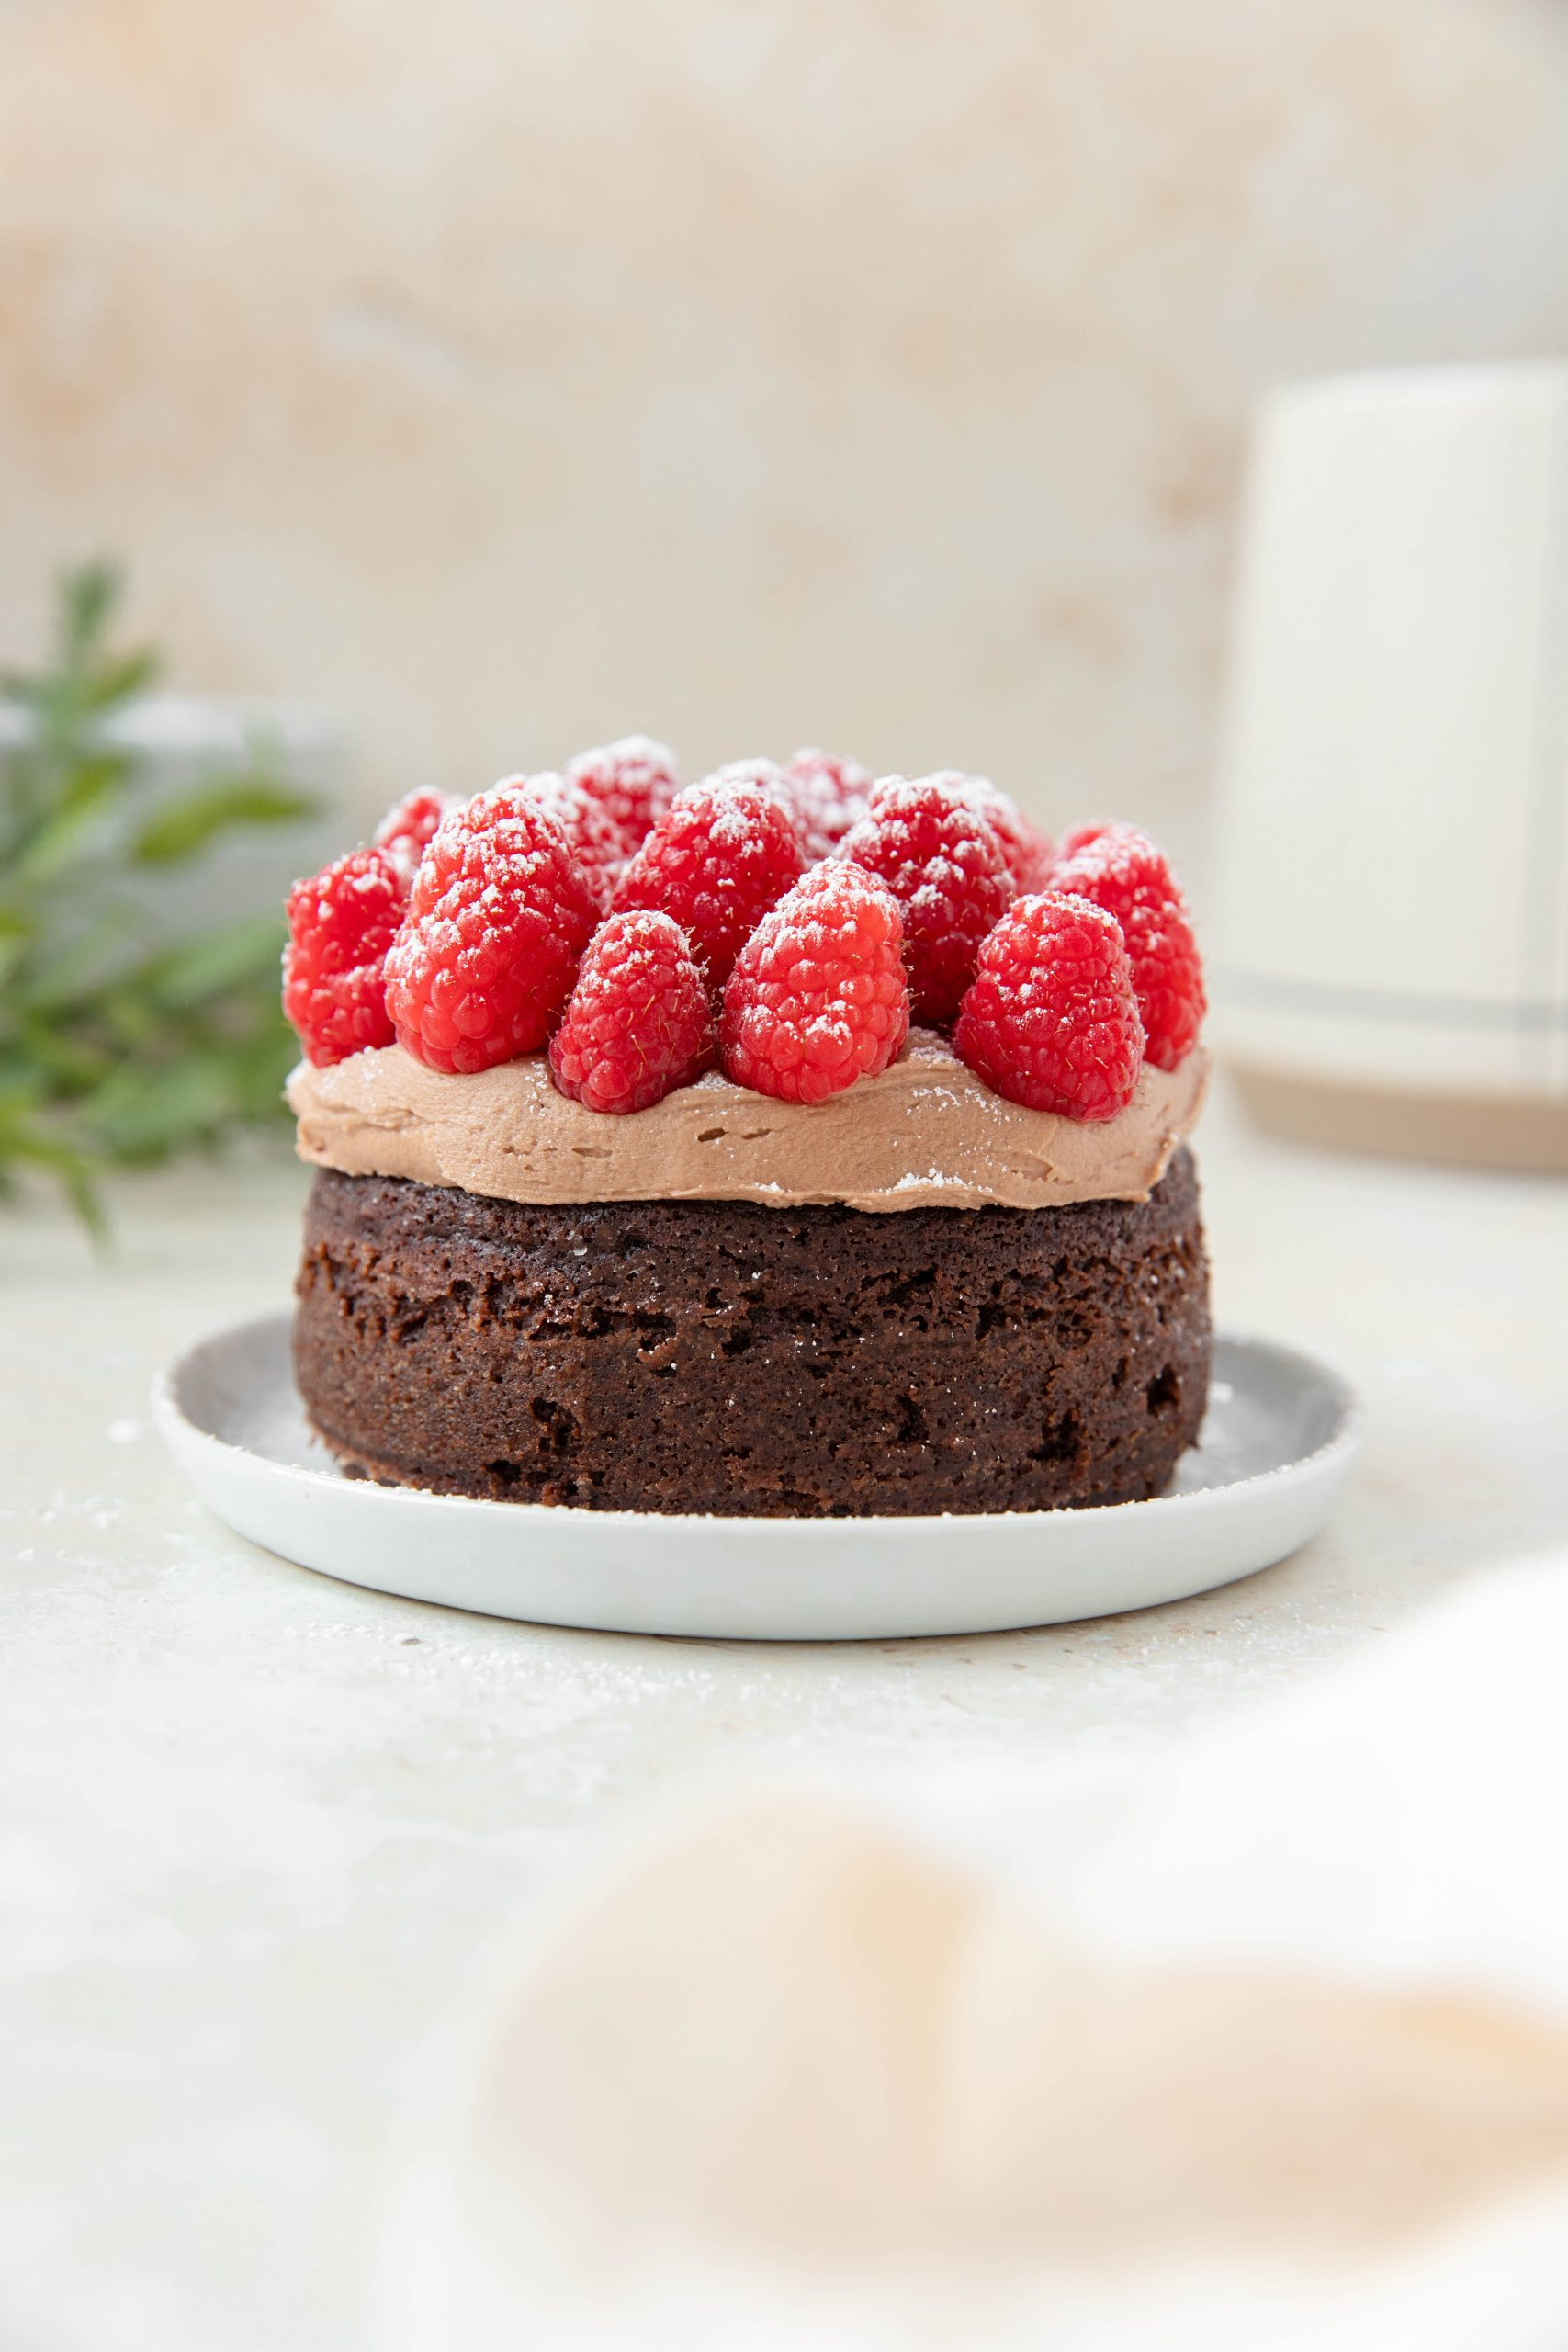
\includegraphics{mcc.jpg}

\begin{longtable}[]{@{}llll@{}}
\toprule\noalign{}
\textbf{PREP TIME} & \textbf{COOK TIME} & \textbf{SERVINGS} &
\textbf{RATING} \\
\midrule\noalign{}
\endhead
\bottomrule\noalign{}
\endlastfoot
15 mins & 15-20 mins & \textbf{1-2} & ★ ★ ★ ★ ★ \\
\end{longtable}

\subsection*{Equipment}\label{equipment-7}
\addcontentsline{toc}{subsection}{Equipment}

\begin{itemize}
\tightlist
\item
  1 4 inch pan
\item
  3 small bowls
\item
  1 medium bowl
\item
  1 hand or stand mixer
\item
  3 whisks
\item
  Cooking spray
\item
  Frosting knife
\end{itemize}

\subsection*{Ingredients}\label{ingredients-7}
\addcontentsline{toc}{subsection}{Ingredients}

Chocolate Cake:

\begin{itemize}
\tightlist
\item
  1/4 cup flour
  \href{https://www.publix.com/pd/publix-all-purpose-flour/RIO-PCI-104014?origin=search1}{*}
\item
  2 tbsp cocoa powder
  \href{https://www.publix.com/pd/hersheys-dutched-cocoa-special-dark/RIO-PCI-102330?origin=search1}{*}
\item
  1/8 tsp baking soda
  \href{https://www.publix.com/pd/arm-and-hammer-baking-soda-pure/RIO-PCI-102907?origin=search1}{*}
\item
  1/8 tsp baking powder
  \href{https://www.publix.com/pd/rumford-baking-powder/RIO-PCI-102919?origin=search1}{*}
\item
  1/8 tsp salt
  \href{https://www.publix.com/pd/morton-salt/RIO-PCI-103677?origin=search9}{*}
\item
  1/4 cup milk
  \href{https://www.publix.com/pd/publix-milk-whole/RIO-PCI-120772?origin=search3}{*}
\item
  1/2 tsp vinegar (white or apple cider)
  \href{https://www.publix.com/pd/publix-vinegar-white-distilled/RIO-PCI-105146?origin=search3}{*}
\item
  2 tbsp olive oil
  \href{https://www.publix.com/pd/publix-olive-oil-extra-virgin/RIO-PCI-103897?origin=search1}{*}
\item
  3 tbsp sugar
  \href{https://www.publix.com/pd/publix-sugar-pure-granulated-extra-fine/RIO-PCI-143101?origin=search1}{*}
\item
  1/2 tsp vanilla extract
  \href{https://www.publix.com/pd/publix-vanilla-extract/RIO-PCI-110432?origin=search1}{*}
\item
  1 tsp hot water
\end{itemize}

Chocolate Frosting:

\begin{itemize}
\tightlist
\item
  3 tbsp butter (slightly softened)
  \href{https://www.publix.com/pd/land-o-lakes-unsalted-butter-made-with-sweet-cream/RIO-PCI-112513?origin=search2}{*}
\item
  3/4 cup powdered sugar
  \href{https://www.publix.com/pd/publix-powdered-sugar-confectioners/RIO-PCI-127078?origin=search1}{*}
\item
  2 tsp cocoa powder
  \href{https://www.publix.com/pd/hersheys-dutched-cocoa-special-dark/RIO-PCI-102330?origin=search1}{*}
\item
  splash of vanilla extract
  \href{https://www.publix.com/pd/publix-vanilla-extract/RIO-PCI-110432?origin=search1}{*}
\item
  1/2-1 tsp milk
  \href{https://www.publix.com/pd/publix-milk-whole/RIO-PCI-120772?origin=search3}{*}
\end{itemize}

Chocolate Frosting:

\begin{itemize}
\tightlist
\item
  15-20 fresh raspberries
  \href{https://www.publix.com/pd/red-raspberries/RIO-PCI-107475?origin=search1}{*}
\item
  powdered sugar
  \href{https://www.publix.com/pd/publix-powdered-sugar-confectioners/RIO-PCI-127078?origin=search1}{*}
\end{itemize}

Click on the '*' next to each ingredient to see detailed information and
resources for it.

Instructions

\textbf{Step 1:} Preheat the oven to 350F. Grease and flour a 4 inch pan
or ramekin (or any 4 inch pan/cup that is oven safe).

\textbf{Step 2:} In a small bowl, combine the flour, cocoa powder,
baking soda, baking powder, and salt. In another small bowl, combine the
milk and vinegar. Stir and let it sit for a couple minutes.

\textbf{Step 3:} While it sits, combine the oil, sugar, and vanilla in a
small bowl. Add the milk/vinegar to the wet ingredients and stir.

\textbf{Step 4:} Pour the dry ingredients into the wet, then gently stir
to combine. Add the hot water and stir again.

\textbf{Step 5:} Pour batter into greased pan, then bake in the oven for
15-20 minutes, until an inserted toothpick comes out clean.

\textbf{Step 6:} While the cake cools, make the frosting. Add the
butter, powdered sugar, and cocoa powder to a medium bowl. Use a hand
mixer (or stand mixer) and mix together for 2 minutes. Add vanilla and
milk and mix again. If you want a thinner frosting, add more milk.

\textbf{Step 7:} When the cake is completely cooled, add the frosting on
top. Top with raspberries, placing them upside down. Finish with a
dusting of powdered sugar. Enjoy!

\chapter*{Ratings and Reviews}\label{ratings-and-reviews}
\addcontentsline{toc}{chapter}{Ratings and Reviews}

\section*{Google Form for Reviews}\label{google-form-for-reviews}
\addcontentsline{toc}{section}{Google Form for Reviews}

Click here to rate the recipes that you have made and tried. You should
only answer the question that corresponds to the recipe you tried.

\href{https://docs.google.com/forms/d/e/1FAIpQLScTyaAdakRAb1C2L7f3DaMqyd_4UnsrQWLYRXmMRr-td62CzQ/viewform?usp=sf_link}{Click
here}

\section*{Interactive Average Ratings
Barplot}\label{interactive-average-ratings-barplot}
\addcontentsline{toc}{section}{Interactive Average Ratings Barplot}

This plot dynamically visualizes the average ratings for each recipe
based on responses submitted via the Google Form. Once you submit your
ratings in the form above, your data will automatically be collected and
stored in a Google Sheet. When the book is re-rendered, it fetches the
latest data from the Google Sheet and displays the updated results for
the average ratings for each recipe. This lets you see the most liked
recipes and dishes based on users' feedback.

\begin{Shaded}
\begin{Highlighting}[]
\CommentTok{\# Load necessary libraries}
\FunctionTok{library}\NormalTok{(ggplot2)}
\FunctionTok{library}\NormalTok{(dplyr)}
\FunctionTok{library}\NormalTok{(readxl)}
\FunctionTok{library}\NormalTok{(googlesheets4)}

\FunctionTok{gs4\_deauth}\NormalTok{()}

\CommentTok{\# Replace with your public Google Sheet URL}
\NormalTok{sheet\_url }\OtherTok{\textless{}{-}} \StringTok{"https://docs.google.com/spreadsheets/d/1LNykmlRDgLpGf85isQpq5OFtFj8Jo0kOfkR0LBC\_1C4/edit"}

\NormalTok{data }\OtherTok{\textless{}{-}} \FunctionTok{read\_sheet}\NormalTok{(sheet\_url)}

\CommentTok{\# Clean the column names (strip leading/trailing spaces)}
\FunctionTok{colnames}\NormalTok{(data) }\OtherTok{\textless{}{-}} \FunctionTok{trimws}\NormalTok{(}\FunctionTok{colnames}\NormalTok{(data))}

\CommentTok{\# Rename columns for simplicity}
\NormalTok{data }\OtherTok{\textless{}{-}}\NormalTok{ data }\SpecialCharTok{\%\textgreater{}\%}
  \FunctionTok{rename}\NormalTok{(}
    \StringTok{\textasciigrave{}}\AttributeTok{Avocado Toast}\StringTok{\textasciigrave{}} \OtherTok{=} \StringTok{\textasciigrave{}}\AttributeTok{How would you rate Avocado Toast w/ Egg?}\StringTok{\textasciigrave{}}\NormalTok{,}
    \StringTok{\textasciigrave{}}\AttributeTok{French Toast}\StringTok{\textasciigrave{}} \OtherTok{=} \StringTok{\textasciigrave{}}\AttributeTok{How would you rate French Toast?}\StringTok{\textasciigrave{}}\NormalTok{,}
    \StringTok{\textasciigrave{}}\AttributeTok{Salmon Rice Bowl}\StringTok{\textasciigrave{}} \OtherTok{=} \StringTok{\textasciigrave{}}\AttributeTok{How would you rate Salmon Rice Bowl?}\StringTok{\textasciigrave{}}\NormalTok{,}
    \StringTok{\textasciigrave{}}\AttributeTok{Turkey Sandwich}\StringTok{\textasciigrave{}} \OtherTok{=} \StringTok{\textasciigrave{}}\AttributeTok{How would you rate Turkey Sandwich?}\StringTok{\textasciigrave{}}\NormalTok{,}
    \StringTok{\textasciigrave{}}\AttributeTok{Garlic Steak Pasta}\StringTok{\textasciigrave{}} \OtherTok{=} \StringTok{\textasciigrave{}}\AttributeTok{How would you rate Garlic Parmesan Steak Pasta?}\StringTok{\textasciigrave{}}\NormalTok{,}
    \StringTok{\textasciigrave{}}\AttributeTok{Brie Burger Tacos}\StringTok{\textasciigrave{}} \OtherTok{=} \StringTok{\textasciigrave{}}\AttributeTok{How would you rate Brie \& Bacon Smash Burger Tacos?}\StringTok{\textasciigrave{}}\NormalTok{,}
    \StringTok{\textasciigrave{}}\AttributeTok{Loaded Brookie}\StringTok{\textasciigrave{}} \OtherTok{=} \StringTok{\textasciigrave{}}\AttributeTok{How would you rate Loaded Brookie?}\StringTok{\textasciigrave{}}\NormalTok{,}
    \StringTok{\textasciigrave{}}\AttributeTok{Chocolate Cake}\StringTok{\textasciigrave{}} \OtherTok{=} \StringTok{\textasciigrave{}}\AttributeTok{How would you rate Mini Chocolate Cake?}\StringTok{\textasciigrave{}}
\NormalTok{  )}

\CommentTok{\# Select only the rating columns}
\NormalTok{ratings }\OtherTok{\textless{}{-}}\NormalTok{ data }\SpecialCharTok{\%\textgreater{}\%}
  \FunctionTok{select}\NormalTok{(}\StringTok{\textasciigrave{}}\AttributeTok{Avocado Toast}\StringTok{\textasciigrave{}}\NormalTok{, }\StringTok{\textasciigrave{}}\AttributeTok{French Toast}\StringTok{\textasciigrave{}}\NormalTok{, }\StringTok{\textasciigrave{}}\AttributeTok{Salmon Rice Bowl}\StringTok{\textasciigrave{}}\NormalTok{, }
         \StringTok{\textasciigrave{}}\AttributeTok{Turkey Sandwich}\StringTok{\textasciigrave{}}\NormalTok{, }\StringTok{\textasciigrave{}}\AttributeTok{Garlic Steak Pasta}\StringTok{\textasciigrave{}}\NormalTok{, }
         \StringTok{\textasciigrave{}}\AttributeTok{Brie Burger Tacos}\StringTok{\textasciigrave{}}\NormalTok{, }\StringTok{\textasciigrave{}}\AttributeTok{Loaded Brookie}\StringTok{\textasciigrave{}}\NormalTok{, }\StringTok{\textasciigrave{}}\AttributeTok{Chocolate Cake}\StringTok{\textasciigrave{}}\NormalTok{)}

\CommentTok{\# Calculate the average ratings for each recipe}
\NormalTok{average\_ratings }\OtherTok{\textless{}{-}} \FunctionTok{colMeans}\NormalTok{(ratings, }\AttributeTok{na.rm =} \ConstantTok{TRUE}\NormalTok{)}

\CommentTok{\# Convert to a data frame for plotting}
\NormalTok{average\_ratings\_df }\OtherTok{\textless{}{-}} \FunctionTok{data.frame}\NormalTok{(}
  \AttributeTok{Recipe =} \FunctionTok{names}\NormalTok{(average\_ratings),}
  \AttributeTok{Average\_Rating =}\NormalTok{ average\_ratings}
\NormalTok{)}

\CommentTok{\# Create the bar plot}
\FunctionTok{ggplot}\NormalTok{(average\_ratings\_df, }\FunctionTok{aes}\NormalTok{(}\AttributeTok{x =} \FunctionTok{reorder}\NormalTok{(Recipe, Average\_Rating), }\AttributeTok{y =}\NormalTok{ Average\_Rating)) }\SpecialCharTok{+}
  \FunctionTok{geom\_bar}\NormalTok{(}\AttributeTok{stat =} \StringTok{"identity"}\NormalTok{, }\AttributeTok{fill =} \StringTok{"skyblue"}\NormalTok{, }\AttributeTok{color =} \StringTok{"black"}\NormalTok{) }\SpecialCharTok{+}
  \FunctionTok{coord\_flip}\NormalTok{() }\SpecialCharTok{+}
  \FunctionTok{labs}\NormalTok{(}
    \AttributeTok{title =} \StringTok{"Average Recipe Ratings"}\NormalTok{,}
    \AttributeTok{x =} \StringTok{"Recipes"}\NormalTok{,}
    \AttributeTok{y =} \StringTok{"Average Rating (1{-}5)"}
\NormalTok{  ) }\SpecialCharTok{+}
  \FunctionTok{theme\_minimal}\NormalTok{() }\SpecialCharTok{+}
  \FunctionTok{theme}\NormalTok{(}
    \AttributeTok{plot.title =} \FunctionTok{element\_text}\NormalTok{(}\AttributeTok{hjust =} \FloatTok{0.5}\NormalTok{, }\AttributeTok{size =} \DecValTok{16}\NormalTok{),}
    \AttributeTok{axis.text =} \FunctionTok{element\_text}\NormalTok{(}\AttributeTok{size =} \DecValTok{12}\NormalTok{),}
    \AttributeTok{axis.title =} \FunctionTok{element\_text}\NormalTok{(}\AttributeTok{size =} \DecValTok{14}\NormalTok{)}
\NormalTok{  )}
\end{Highlighting}
\end{Shaded}

\includegraphics{_main_files/figure-latex/helper-1.pdf}

```

\chapter*{References}\label{references}
\addcontentsline{toc}{chapter}{References}

\begin{enumerate}
\def\labelenumi{\arabic{enumi}.}
\item
  Collins, Nicole. ``Food Blog: United States: The Yummy Muffin.''
  \emph{Yummy Muffin}, 29 Nov.~2024,
  \href{https://www.theyummymuffin.com/}{www.theyummymuffin.com}.
\item
  Dingwall, Holly. ``Foodieholly's Recipes from around the World.''
  \emph{Foodieholly}, 29 Nov.~2024,
  \href{https://foodieholly.com/}{foodieholly.com}.
\item
  Gritzer, Daniel. ``Perfect Quick-and-Easy French Toast Recipe.''
  \emph{Serious Eats}, Serious Eats, 5 Nov.~2024,
  \href{https://www.seriouseats.com/perfect-quick-easy-french-toast}{www.seriouseats.com/perfect-quick-easy-french-toast}.
\item
  Oniki, Mallory. ``The Palatable Life.'' \emph{The Palatable Life}, 2
  Apr.~2021,
  \href{https://www.thepalatablelife.com/}{www.thepalatablelife.com}.
\item
  Rivers, Alyssa. \emph{The Recipe Critic}, 25 Nov.~2024,
  \href{https://www.therecipecritic.com/}{www.therecipecritic.com}.
\item
  Xie, Yihui. ``Authoring Books and Technical Documents with R
  Markdown.'' Bookdown, 25 Oct.~2024,
  \href{https://bookdown.org/yihui/bookdown/}{www.bookdown.org}.
\end{enumerate}

\backmatter
\end{document}
